\documentclass[paper=a4, fontsize=12pt]{scrartcl}

\usepackage[bottom=1.6in, right=0.9in]{geometry}
\usepackage[brazil]{babel} % pacote portugues brasileiro
\usepackage[utf8]{inputenc} % pacote para acentuacao direta
\usepackage[T1]{fontenc} % Use 8-bit encoding that has 256 glyphs
%\usepackage{fourier} % Use the Adobe Utopia font for the document - comment this line to return to the LaTeX default
%\usepackage[english]{babel} % English language/hyphenation
\usepackage{amsmath,amsfonts,amsthm} % Math packages

\usepackage{float}
\usepackage{xtab}
\usepackage{tabularx}
\usepackage{graphicx}
\setlength{\parskip}{1em}
\usepackage{color}
\usepackage[table]{colortbl}
\usepackage{sourcecodepro}

\usepackage{fancyvrb}
\RecustomVerbatimCommand{\VerbatimInput}{VerbatimInput}
{fontsize=\scriptsize,
	%
	frame=lines,  % top and bottom rule only
	framesep=2em, % separation between frame and text
	rulecolor=\color{Gray},
	%
	label=\fbox{\color{Black}Resultado},
	labelposition=topline,
	%
	%commandchars=\|\(\), % escape character and argument delimiters for
	% commands within the verbatim
	commentchar=*        % comment character
}
\usepackage[usenames,dvipsnames,svgnames,table]{xcolor}
\definecolor{gray}{HTML}{212121}
\usepackage{listings}
%\usepackage{listingsutf8}
\lstset{
	breaklines=true,
	numbers=left,
	numberstyle=\tiny,
	basicstyle=\ttfamily\footnotesize,
}
\lstset{
	inputencoding=utf8,
	extendedchars=true,
	captionpos=b,
	literate=%
	{é}{{\'{e}}}1
	{è}{{\`{e}}}1
	{ê}{{\^{e}}}1
	{ë}{{\¨{e}}}1
	{É}{{\'{E}}}1
	{Ê}{{\^{E}}}1
	{û}{{\^{u}}}1
	{ù}{{\`{u}}}1
	{ú}{{\'{u}}}1
	{â}{{\^{a}}}1
	{à}{{\`{a}}}1
	{á}{{\'{a}}}1
	{ã}{{\~{a}}}1
	{Á}{{\'{A}}}1
	{Â}{{\^{A}}}1
	{Ã}{{\~{A}}}1
	{ç}{{\c{c}}}1
	{Ç}{{\c{C}}}1
	{õ}{{\~{o}}}1
	{ó}{{\'{o}}}1
	{ô}{{\^{o}}}1
	{Õ}{{\~{O}}}1
	{Ó}{{\'{O}}}1
	{Ô}{{\^{O}}}1
	{î}{{\^{i}}}1
	{Î}{{\^{I}}}1
	{í}{{\'{i}}}1
	{Í}{{\~{Í}}}1
}
\renewcommand{\lstlistingname}{Código}


\usepackage{sectsty} % Allows customizing section commands
\allsectionsfont{\normalfont\scshape\bfseries} % Make all sections centered, the default font and small caps

\usepackage{fancyhdr} % Custom headers and footers
\pagestyle{fancyplain} % Makes all pages in the document conform to the custom headers and footers
\fancyhead{} % No page header - if you want one, create it in the same way as the footers below
\fancyfoot[L]{} % Empty left footer
\fancyfoot[C]{} % Empty center footer
\fancyfoot[R]{\thepage} % Page numbering for right footer
\renewcommand{\headrulewidth}{0pt} % Remove header underlines
\renewcommand{\footrulewidth}{0pt} % Remove footer underlines
\setlength{\headheight}{13.6pt} % Customize the height of the header

\numberwithin{equation}{section} % Number equations within sections (i.e. 1.1, 1.2, 2.1, 2.2 instead of 1, 2, 3, 4)
\numberwithin{figure}{section} % Number figures within sections (i.e. 1.1, 1.2, 2.1, 2.2 instead of 1, 2, 3, 4)
\numberwithin{table}{section} % Number tables within sections (i.e. 1.1, 1.2, 2.1, 2.2 instead of 1, 2, 3, 4)

\setlength\parindent{0pt} % Removes all indentation from paragraphs - comment this line for an assignment with lots of text


\newcommand{\euler}{e}
%----------------------------------------------------------------------------------------
%	TITLE SECTION
%----------------------------------------------------------------------------------------

\newcommand{\horrule}[1]{\rule{\linewidth}{#1}} % Create horizontal rule command with 1 argument of height

\title{
	\normalfont \normalsize
	%\textsc{UNIVERSIDADE TECNOLÓGICA FEDERAL DO PARANÁ} \\ [15pt] % Your university, school and/or department name(s)
	\horrule{0.5pt} \\[0.4cm] % Thin top horizontal rule
	\huge Cálculo numérico: lista de exercícios\\ % The assignment title
	\Large Lucas Rafael Gris \\
	\Large Turma: A41 \\
	%\date{\normalsize\today} % Today's date or a custom date
	\horrule{0.5pt} \\[0.5cm] % Thick bottom horizontal rule
}
\date{Maio, 2017}

\newcommand*{\titleGM}{
	\thispagestyle{empty}
	\begingroup % Create the command for including the title page in the document
	\hbox{ % Horizontal box
		\hspace*{0.2\textwidth} % Whitespace to the left of the title page
		\rule{1pt}{\textheight} % Vertical line
		\hspace*{0.05\textwidth} % Whitespace between the vertical line and title page text
		\parbox[b]{0.75\textwidth}{ % Paragraph box which restricts text to less than the width of the page
			{\noindent\Huge\bfseries Cálculo numérico \\}\\[2\baselineskip] % Title
			{\large \textit{\textbf{Nome:} Lucas Rafael Gris\ \ \ \ \textbf{RA: 1640496} \ \ \ \ \textbf{Turma:} A41}}\\[1\baselineskip]
			{\large \textbf{Tema:} Lista de Exercícios } \\[4\baselineskip] % Tagline or further description
			{\large \textsc{Maio de 2017} }
			%{\large \textsc{ Prof. Diego Venâncio Thomaz}} % Author name

			\vspace{0.5\textheight} % Whitespace between the title block and the publisher
			{\noindent Universidade Técnologica Federal do Paraná \\ Campus Medianeira }\\[\baselineskip] % Publisher and logo
		}}
		\endgroup}



\begin{document}

\titleGM

\section*{Algoritmos}

	A seguir apresenta-se algoritmos desenvolvidos em \textit{Python} para a resolução de alguns exercícios. 

	\hspace{2cm}

	\lstinputlisting[language=Python, caption= {Métodos de integração numérica em \textit{Python}}]{algorithms/integrmethods.py}

	\lstinputlisting[language=Python, caption= {Métodos de resolução de EDO em \textit{Python}}]{algorithms/odemethods.py}

	\newpage

\section*{Lista de exercícios 5}

	\subsection{Exercício 1}\label{ex01}

		Estamos interessados em aplicar a regra do trapézio para calcular $\int_{1.00}^{1.30} \sqrt{x} dx$ utilizando os seguintes pontos:

		\begin{table}[H]
			\def\arraystretch{1.5}
			\begin{center}
				\caption{Pontos $\sqrt{x}$}
				\label{points_ex01}
				\begin{tabularx}
					{\textwidth}{|X|p{1.5cm}|p{1.5cm}|p{1.5cm}|p{1.5cm}|p{1.5cm}|p{1.5cm}|p{1.5cm}|}
					\hline
					{$x$} & 1.00 & 1.05 & 1.10 & 1.15 & 1.20 & 1.25 & 1.30 \\
					\hline
					{$\sqrt{x}$} & 1.0000 & 1.0247 & 1.0488 & 1.0723 & 1.0954 & 1.1180 & 1.1401 \\
					\hline
				\end{tabularx}
			\end{center}
		\end{table}

		Sabemos que:

		\begin{align*}
			\begin{split}
				\int_{x_1}^{x_n} f(x) dx 	&= \int_{x_0}^{x_1} f(x) + \int_{x_1}^{x_2} f(x) + \ldots + \int_{x_{n-1}}^{x_n} f(x) \\
																	&= \frac{h}{2}\left[ f(x_0) + f(x_1) \right] + \frac{h}{2}\left[ f(x_1) + f(x_3) \right] + \ldots + \frac{h}{2}\left[ f(x_{n-1}) + f(x_n) \right] \\
																	&= \frac{h}{2}\left[ f(x_0) + 2\cdot (f(x_1) + f(x_2) + \ldots  + f(x_{n-1})) + f(x_n) \right]
			\end{split}
		\end{align*}

		Então aplicando nos pontos em \ref{points_ex01} obtemos:

		\begin{align*}
		\begin{split}
		\int_{1.00}^{1.30} \sqrt{x} dx 	&= \frac{0.05}{2}\left[ 1.0000  + 2\cdot (1.0247 + 1.0488 + 1.0723 + 1.0954 + 1.1180) + 1.1401 \right] \\
																	&=  \frac{0.05}{2}\left[ 1.0000  + (10.7184) + 1.1401 \right] \\
																	&=  0.3214625
		\end{split}
		\end{align*}


		\subsection{Exercício 2}\label{ex02}

		Queremos calcular $\int_{0}^{0.8} \cos{(x)} dx$ utilizando a regra do trapézio, com $h = 0.4, 0.2 $ e $0.1$, para os seguintes pontos:

		\begin{table}[H]
			\def\arraystretch{1.5}
			\begin{center}
				\caption{Pontos $\cos{x}$}
				\label{points_ex02}
				\begin{tabularx}
					{\textwidth}{|X|p{1.1cm}|p{1.1cm}|p{1.1cm}|p{1.1cm}|p{1.1cm}|p{1.1cm}|p{1.1cm}|p{1.1cm}|p{1.1cm}|}
					\hline
					{$x$} & 0 & 0.1 & 0.2 & 0.3 & 0.4 & 0.5 & 0.6 & 0.7 & 0.8 \\
					\hline
					{$\cos{(x)}$} & 1 & 0.995 & 0.980 & 0.955 & 0.921  & 0.877 & 0.825 & 0.764 & 0.696 \\
					\hline
				\end{tabularx}
			\end{center}
		\end{table}

		Para $h = 0.4$ temos:

		\begin{align*}
			\begin{split}
				\int_{0}^{0.8} \cos{(x)} dx 	&= \frac{0.4}{2}\left[ 1  + 2\cdot (0.921) + 0.696 \right] =  \frac{0.4}{2}\left[ 1  + (1.842) + 0.696 \right] \\
				&=  0.7076
			\end{split}
		\end{align*}

		Para $h = 0.2$ temos:

		\begin{align*}
			\begin{split}
				\int_{0}^{0.8} \cos{(x)} dx &= \frac{0.2}{2}\left[ 1  + 2\cdot (0.980 + 0.921 + 0.825) + 0.696 \right] =  \frac{0.4}{2}\left[ 1  + (5.452) + 0.696 \right] \\
				&= 0.7248
			\end{split}
		\end{align*}

		Para $h = 0.1$ temos:

		\begin{align*}
		\begin{split}
		\int_{0}^{0.8} \cos{(x)} dx 	&= \frac{0.1}{2}\left[ 1  + 2\cdot (0.995 + 0.980 + 0.955 + 0.921 + 0.877 + 0.825 + 0.764) + 0.696 \right] \\
																	&=  \frac{0.1}{2}\left[ 1  + (12.64) + 0.696 \right] \\
																	&=  0.7168
		\end{split}
		\end{align*}

		\subsection{Exercício 3}

		Estamos interessados em obter o valor das integrais definidas discutidas em \ref{ex01} e \ref{ex02} através da regra de $ \frac{1}{3} $ de \textit{Simpson} e da integral discutida em \ref{ex01} utilizando a regra $  \frac{3}{8} $ de \textit{Simpson}.

		Para $\int_{1.00}^{1.30} \sqrt{x} dx$ e utilizando a regra de $ \frac{1}{3} $ de \textit{Simpson} temos:

		\begin{align*}
			\begin{split}
			\int_{x_0}^{x_{2n}} f(x) dx 	&= \int_{x_0}^{x_2} f(x) + \int_{x_2}^{x_4} f(x) + \ldots + \int_{x_{2n-2}}^{x_{2n}} f(x) \\
			&= \frac{h}{3}\left[ f(x_0) + 4f(x_1) + f(x_2)\right] + \frac{h}{3}\left[ f(x_2) + 4f(x_3) + f(x_4) \right] + \ldots \\&+ \frac{h}{3}\left[ f(x_{2n-2}) + 4f(x_{2n-1}) + f(x_{2n}) \right] \\
			&= \frac{h}{3}\left[ f(x_0) + 4f(x_1) + 2f(x_2) + 4f(x_3) + \ldots + 2f(x_{2n-2}) + 4f(x_{2n-1}) + f(x_{2n}) \right]
			\end{split}
		\end{align*}

		Note que para aplicarmos a regra de \textit{Simpson} temos que obrigatoriamente utilizar $2n + 1$ pontos. Assim, utilizaremos todos os pontos de \ref{points_ex01} para obter uma solução da integral definida.

		\begin{align*}
			\begin{split}
				2n + 1 = 7 	&\implies \quad n = 3 \\
										&\implies h = \frac{b - a}{2n} = \frac{1.30 - 1.00}{6} = \frac{0.3}{6}\\
			\end{split}
		\end{align*}

		para \ref{ex01}, para \ref{ex02} temos:

		\begin{align*}
			\begin{split}
				2n + 1 = 9 	&\implies \quad n = 4 \\
				&\implies h = \frac{b - a}{2n} = \frac{0.8 - 0.0}{8} = \frac{0.8}{8}\\
			\end{split}
		\end{align*}

		Logo,

		\begin{align*}
			\begin{split}
				\int_{1.00}^{1.30} \sqrt{x} dx
				&= \frac{h}{3}\left[ f(x_0) + 4f(x_1) + 2f(x_2) + 4f(x_3) + \ldots + 2f(x_{2n-2}) + 4f(x_{2n-1}) + f(x_{2n}) \right] \\
				&= \frac{0.3}{18}\left[ 1.0000 + 4(1.0247 + 1.0723 + 1.1180) + 2(1.0488 + 1.0954) + 1.1401) \right] \\
				&= \frac{0.3}{18}\left[ 1.0000 + 4(3.215) + 2(2.1447) + 1.1401) \right] \\
				&= 0.3215
			\end{split}
		\end{align*}

		\begin{align*}
			\begin{split}
				\int_{0}^{0.8} \cos{x} dx
				&= \frac{h}{3}\left[ f(x_0) + 4f(x_1) + 2f(x_2) + 4f(x_3) + \ldots + 2f(x_{2n-2}) + 4f(x_{2n-1}) + f(x_{2n}) \right] \\
				&= \frac{0.8}{24}\left[ 1 + 4(0.995 + 0.955 + 0.877 + 0.764) + 2(0.980 + 0.921 + 0.825) + 0.696) \right] \\
				&= \frac{0.8}{24}\left[ 1 + 4(3.591) + 2(2.726) + 0.696) \right] \\
				&= 0.7170
			\end{split}
		\end{align*}

		De forma análoga, queremos calcular $ \int_{1.00}^{1.30} \sqrt{x} dx $ pela regra $\frac{3}{8}$ de \textit{Simpson}. Neste caso temos que utilizar $3n + 1$ pontos.

		Assim,

		\begin{align*}
			\begin{split}
				3n + 1 = 7 	&\implies \quad n = 2 \\
				&\implies h = \frac{b - a}{3n} = \frac{1.30 - 1.00}{6} = \frac{0.3}{6}\\
			\end{split}
		\end{align*}

		Logo,

		\begin{align*}
			\begin{split}
				\int_{1.00}^{1.30} \sqrt{x} dx
				&= \frac{3h}{8}[ f(x_0) + 3f(x_1) + 3f(x_2) + 2f(x_3) + \ldots \\
				&+ 2f(x_{3n-3}) + 3f(x_{3n-2}) + 3f(x_{3n-1}) + f(x_{3n})] \\
				&= \frac{0.9}{48}\left[ 1.0000 + 3(1.0247 + 1.0488 + 1.0954 + 1.1180) + 2(1.0723) + 1.1401 \right] \\
				&= \frac{0.9}{48}\left[ 1.0000 + 3(4.2869) + 2(1.0723) + 1.1401 \right]\\
				&= 0.32147 \\
			\end{split}
		\end{align*}

		\subsection{Exercício 4}

		Dada a integral definida

		\begin{align*}
			\begin{split}
			\int_{0}^{1} t^{3}\euler^{t} dt
			\end{split}
		\end{align*}

		Queremos obter a solução da mesma através dos métodos do Trapézio e a Regra 1/3 de \textit{Simpson} utilizando uma distancia $h$ entre os pontos de $ 0.5 $ e $ 0.25 $ .

		Para isso obteremos os valores da função $f(t) = t^{3}\euler^{t}$ em $[0, 1]$ utilizando um intervalo de $0.25$ entre os pontos.

 		\begin{table}[H]
 			\def\arraystretch{1.5}
 			\begin{center}
 				\caption{Pontos $t^{3}\euler^{t}$}
 				\label{points_ex04}
 				\begin{tabularx}
 					{\textwidth}{|X|p{2cm}|p{2cm}|p{2cm}|p{2cm}|p{2cm}|}
 					\hline
 					{$t$} & 0 & 0.25 & 0.5 & 0.75 & 1 \\
 					\hline
 					{$f{(t)}$} & 0 & 0.0020062 & 0.206090 & 0.893109 & 2.718281 \\
 					\hline
 				\end{tabularx}
 			\end{center}
 		\end{table}

		Para $h = 0.5$, utilizando a Regra do Trapézio:


		\begin{align*}
			\begin{split}
				\int_{0}^{1} t^{3}\euler^{t} dt &= \frac{0.5}{2}\left[0 + 2(0.206090) + 2.718281 \right]\\ &=  \frac{0.5}{2}\left[(0.41218) + 2.718281 \right] \\
				&= 0.782615
			\end{split}
		\end{align*}

		Com $h = 0.25$, e utilizando a Regra do Trapézio obtemos:

		\begin{align*}
			\begin{split}
				\int_{0}^{1} t^{3}\euler^{t} dt &= \frac{0.25}{2}\left[0 + 2(0.0020062 + 0.206090 + 0.893109) + 2.718281 \right]\\ &=  \frac{0.25}{2}\left[(1.1012052) + 2.718281 \right] \\
				&= 0.615085
			\end{split}
		\end{align*}

		Para $h = 0.5$, utilizando a Regra 1/3 de \textit{Simpson}:


		\begin{align*}
			\begin{split}
				\int_{0}^{1} t^{3}\euler^{t} dt &= \frac{0.5}{3}\left[0 + 4(0.206090) + 2.718281 \right]\\ &=  \frac{0.5}{3}\left[(0.82436) + 2.718281 \right] \\
				&= 0.59044
			\end{split}
		\end{align*}

		Com $h = 0.25$, e utilizando a Regra 1/3 de \textit{Simpson} obtemos:

		\begin{align*}
			\begin{split}
				\int_{0}^{1} t^{3}\euler^{t} dt &= \frac{0.25}{3}\left[0 + 4(0.0020062 + 0.893109) + 2(0.206090) + 2.718281 \right]\\ &=  \frac{0.25}{3}\left[4(0.8951152) + 2(0.41218) + 2.718281 \right] \\
				&= 0.5592
			\end{split}
		\end{align*}

		\subsection{Exercício 5}

		A fórmula de \textit{Newton-Cotes} é exata para polinômios de grau n, onde n é o grau do polinômio usado na interpolação para a obtenção da fórmula de integração.

		Por exemplo, no caso de uma aproximação do tipo:

		\begin{align*}
			\begin{split}
				\int_{a}^{b} f(x) dx \approx \int_{a}^{b} P_n(x) dx &= \sum_{k=0}^{n} f_k \cdot h \cdot C_k^n
			\end{split}
		\end{align*}

		O cálculo para a integral definida de $P_n(x)$ é exato. Para a Regra $ \frac{3}{8} $ de \textit{Simpson}, o cálculo é exato caso a função utilizada seja uma função de grau três.

		\textbf{Exemplo}. Considere $P_3(x) = x^3$ e o intervalo [0, 1], analiticamente temos:

		\begin{align*}
			\begin{split}
				\int_{0}^{1} x^3 dx &= \frac{1}{4}x^4 \Big|_0^1 = \frac{1}{4}
			\end{split}
		\end{align*}

		E por \textit{Newton-Cotes} (Regra $ \frac{3}{8} $ de \textit{Simpson}), temos:

		\begin{align*}
			\begin{split}
				h = \frac{1 - 0}{3} = \frac{1}{3} \quad &\implies \quad x_0 = 0,\ x_1 = \frac{1}{3},\ x_2 = \frac{2}{3},\ x_3 = 1
			\end{split}
		\end{align*}

		Assim,

		\begin{align*}
			\begin{split}
				\int_{0}^{1} x^3 dx &= \frac{3}{8} \cdot \Big(\frac{1}{3}\Big) \cdot \Big[0 + 3\frac{1}{27} + 3\frac{8}{27} + 1\Big] \\
				&= \frac{1}{8} \Big[  2 \Big] \\
				&= \frac{1}{4}
			\end{split}
		\end{align*}

		\subsection{Exercício 6}

		Estamos interessados em calcular $ \int_{0}^{1.2}\euler^{-x}\sin(x) $ através da Regra $ \frac{3}{8} $ de \textit{Simpson}. Sabemos que:

		\begin{table}[H]
			\def\arraystretch{1.5}
			\begin{center}
				\caption{Pontos $\euler^{-x} \ $e $\ \sin(x)$}
				\label{points_ex06}
				\begin{tabularx}
					{\textwidth}{|X|p{1.5cm}|p{1.5cm}|p{1.5cm}|p{1.5cm}|p{1.5cm}|p{1.5cm}|p{1.5cm}|}
					\hline
					{$x$} & 0 & 0.2 	 & 0.4  & 0.6  & 0.8  & 1.0  & 1.2 \\
					\hline
					{$\euler^{-x}$} & 1.000 & 0.819  & 0.670 & 0.548  & 0.449  & 0.367 & 0.301 \\
					\hline
					{$\sin(x)$} & 0 & 0.198 & 0.398  & 0.565 & 0.717   & 0.841  & 0.932 \\
					\hline
				\end{tabularx}
			\end{center}
		\end{table}

		Então é suficiente obter a fórmula da regra de \textit{Simpson} e aplicar os pontos da função $f$ obtidos através do produto entre $\euler^{-x} \ $e $\ \sin(x)$.

		Considerando $h = 0.4$ temos que:

		\begin{align*}
			\begin{split}
				3n + 1 = 4 	&\implies \quad n = 1 \\
				&\implies h = \frac{b - a}{3n} = \frac{1.2 - 0}{3} = \frac{1.2}{3}\\
			\end{split}
		\end{align*}

		Logo,

		\begin{align*}
			\begin{split}
				\int_{0}^{1.2} \euler^{-x}\sin(x)  dx &= \frac{3h}{8}[ f(x_0) + 3f(x_1) + 3f(x_2) + f(x_3)] \\
				&= \frac{1.2}{8}\left[0 + 3(0.26666 + 0.321933) + 0.290532) \right] \\
				&= \frac{1.2}{8}\left[ 2.056311 \right]\\
				&=  0.30844665\\
			\end{split}
		\end{align*}

		E considerando $h = 0.2$ obtemos:

		\begin{align*}
			\begin{split}
				3n + 1 = 7 	&\implies \quad n = 2 \\
				&\implies h = \frac{b - a}{3n} = \frac{1.2 - 0}{6} = \frac{1.2}{6}\\
			\end{split}
		\end{align*}

		Logo,

		\begin{align*}
			\begin{split}
				\int_{0}^{1.2} \euler^{-x}\sin(x)  dx &= \frac{3h}{8}[ f(x_0) + 3[f(x_1) + f(x_2) + f(x_4) + f(x_5)] + 2f(x_3) + f(x_6)] \\
				&= \frac{3.6}{48}\left[0 + 3(0.16212 + 0.26666 + 0.321933 + 0.308647) +  2(0.30962) +  0.280532\right] \\
				&= \frac{3.6}{48}\left[3.17808 + 0.61924 + 0.280532 \right]\\
				&=  0.3058389\\
			\end{split}
		\end{align*}

		\subsection{Execício 7}\label{ex07}

		Estamos interessados em definir um intervalo igualmente espaçado $h$ para o cálculo da integral definida utilizando a Regra do Trapézio, tal que o valor de $\int_{0}^{1} \euler^{-x^2}$ tenha um erro inferior a $0.5 \times 10^{-6}$.

		\begin{align*}
			\begin{split}
				| R(f) | \leq \frac{b - a}{12} \times h^2 \times \max_{a \leq t \leq b} |f^{''}(t)| & < 0.5 \times 10^{-6}\\ \implies \quad h^2  &< \frac{0.5 \times 10^{-6}}{\frac{b - a}{12} \times \max_{a \leq t \leq b} |f^{''}(t)|}
			\end{split}
		\end{align*}


		\begin{align*}
			\begin{split}
				f^{'} (x) &= -2x\euler^{-x^2} \\
				f^{''} (x) &= 4x^2\euler^{-x^2} - 2\euler^{-x^2} = (4x^2 -2)\euler^{-x^2}\\
			\end{split}
		\end{align*}

		A função $ f^{''}(x) $ é sempre crescente no intervalo (0, 1), logo:

		\begin{align*}
			\begin{split}
				\max_{0 \leq t \leq 1} |f^{''}(t)| = |f^{''} (1)| &= 0.7357588\\
			\end{split}
		\end{align*}

		Portanto,

		\begin{align*}
			\begin{split}
				h^2  	&< \frac{0.5 \times 10^{-6}}{\frac{1}{12} \times 0.7357588} \\
				h^2 	&< 8.15 \times 10^{-6} \\
				h 		&< 2.85566 \times 10^{-3}
			\end{split}
		\end{align*}

		Para encontrarmos um valor exato de $h$ que satisfaça a condição, devemos obter o valor máximo de $h$ tal que $ h < 2.85566 \times 10^{-3} $ seja satisfeita e seja possível obtermos todos os pontos necessários no intervalo [0, 1].

		Note que o espaçamento $h$ é dado por:

		\begin{align*}
			h = \frac{b - a}{N}
		\end{align*}

		onde $N + 1$ é a quantidade de pontos utilizados na aplicação da regra do Trapézio. Assim:

		\begin{align*}
		h = \frac{b - a}{N} < 2.85566 \times 10^{-3}\implies N &> \frac{1}{2.85566 \times 10^{-3}} \\
		 N &> 350.181744  \\
		\end{align*}

		que não é um número inteiro. Logo devemos encontrar um valor $h$ tal que:

		\begin{align*}
		\frac{b - a}{h} = \frac{1}{h} = 351
		\end{align*}

		De fato,

		\begin{align*}
			\quad  h = 0.002849002849 < 2.85566 \times 10^{-6}
		\end{align*}

		Portanto um intervalo igualmente espaçado $h = 0.002849002849$ entre os pontos satisfaz o erro desejado num total de 352 pontos.

		\textbf{Cálculo da integral.} O valor da integral pode ser calculado utilizando os algoritmos desenvolvidos em \textit{Python} e em C:

		\hspace{2cm}

		\lstinputlisting[language=Python, caption= Cálculo em \textit{Python}]{algorithms/ex07-1.py}

		\hspace{2cm}

		\lstinputlisting[language=C, caption= Cálculo de integral pela regra do Trapézio em \textit{C}]{algorithms/trapezoidal.c}

		Onde obtemos os valores $0.746823635144$ e $0.7468236351$	respectivamente.

		\subsection{Exercício 8}

		Queremos calcular $\int_{1}^{2} \frac{\euler^x}{x} dx$ com erro inferior a $ 0.05 $, usando a regra do Trapézio.

		\begin{align*}
			\begin{split}
				| R(f) | \leq \frac{b - a}{12} \times h^2 \times \max_{a \leq t \leq b} |f^{''}(t)| & < 0.05\\ \implies \quad h^2  &< \frac{0.05}{\frac{b - a}{12} \times \max_{a \leq t \leq b} |f^{''}(t)|}
			\end{split}
		\end{align*}


		\begin{align*}
			\begin{split}
				f^{'} (x) &= \frac{\euler^{x}(x - 1) }{x^{2}}\\
				f^{''} (x) &= \frac{\euler^{x}(x^2 -2x + 2)}{x^3}\\
			\end{split}
		\end{align*}

 		\begin{figure}[H]
 			\centering
 			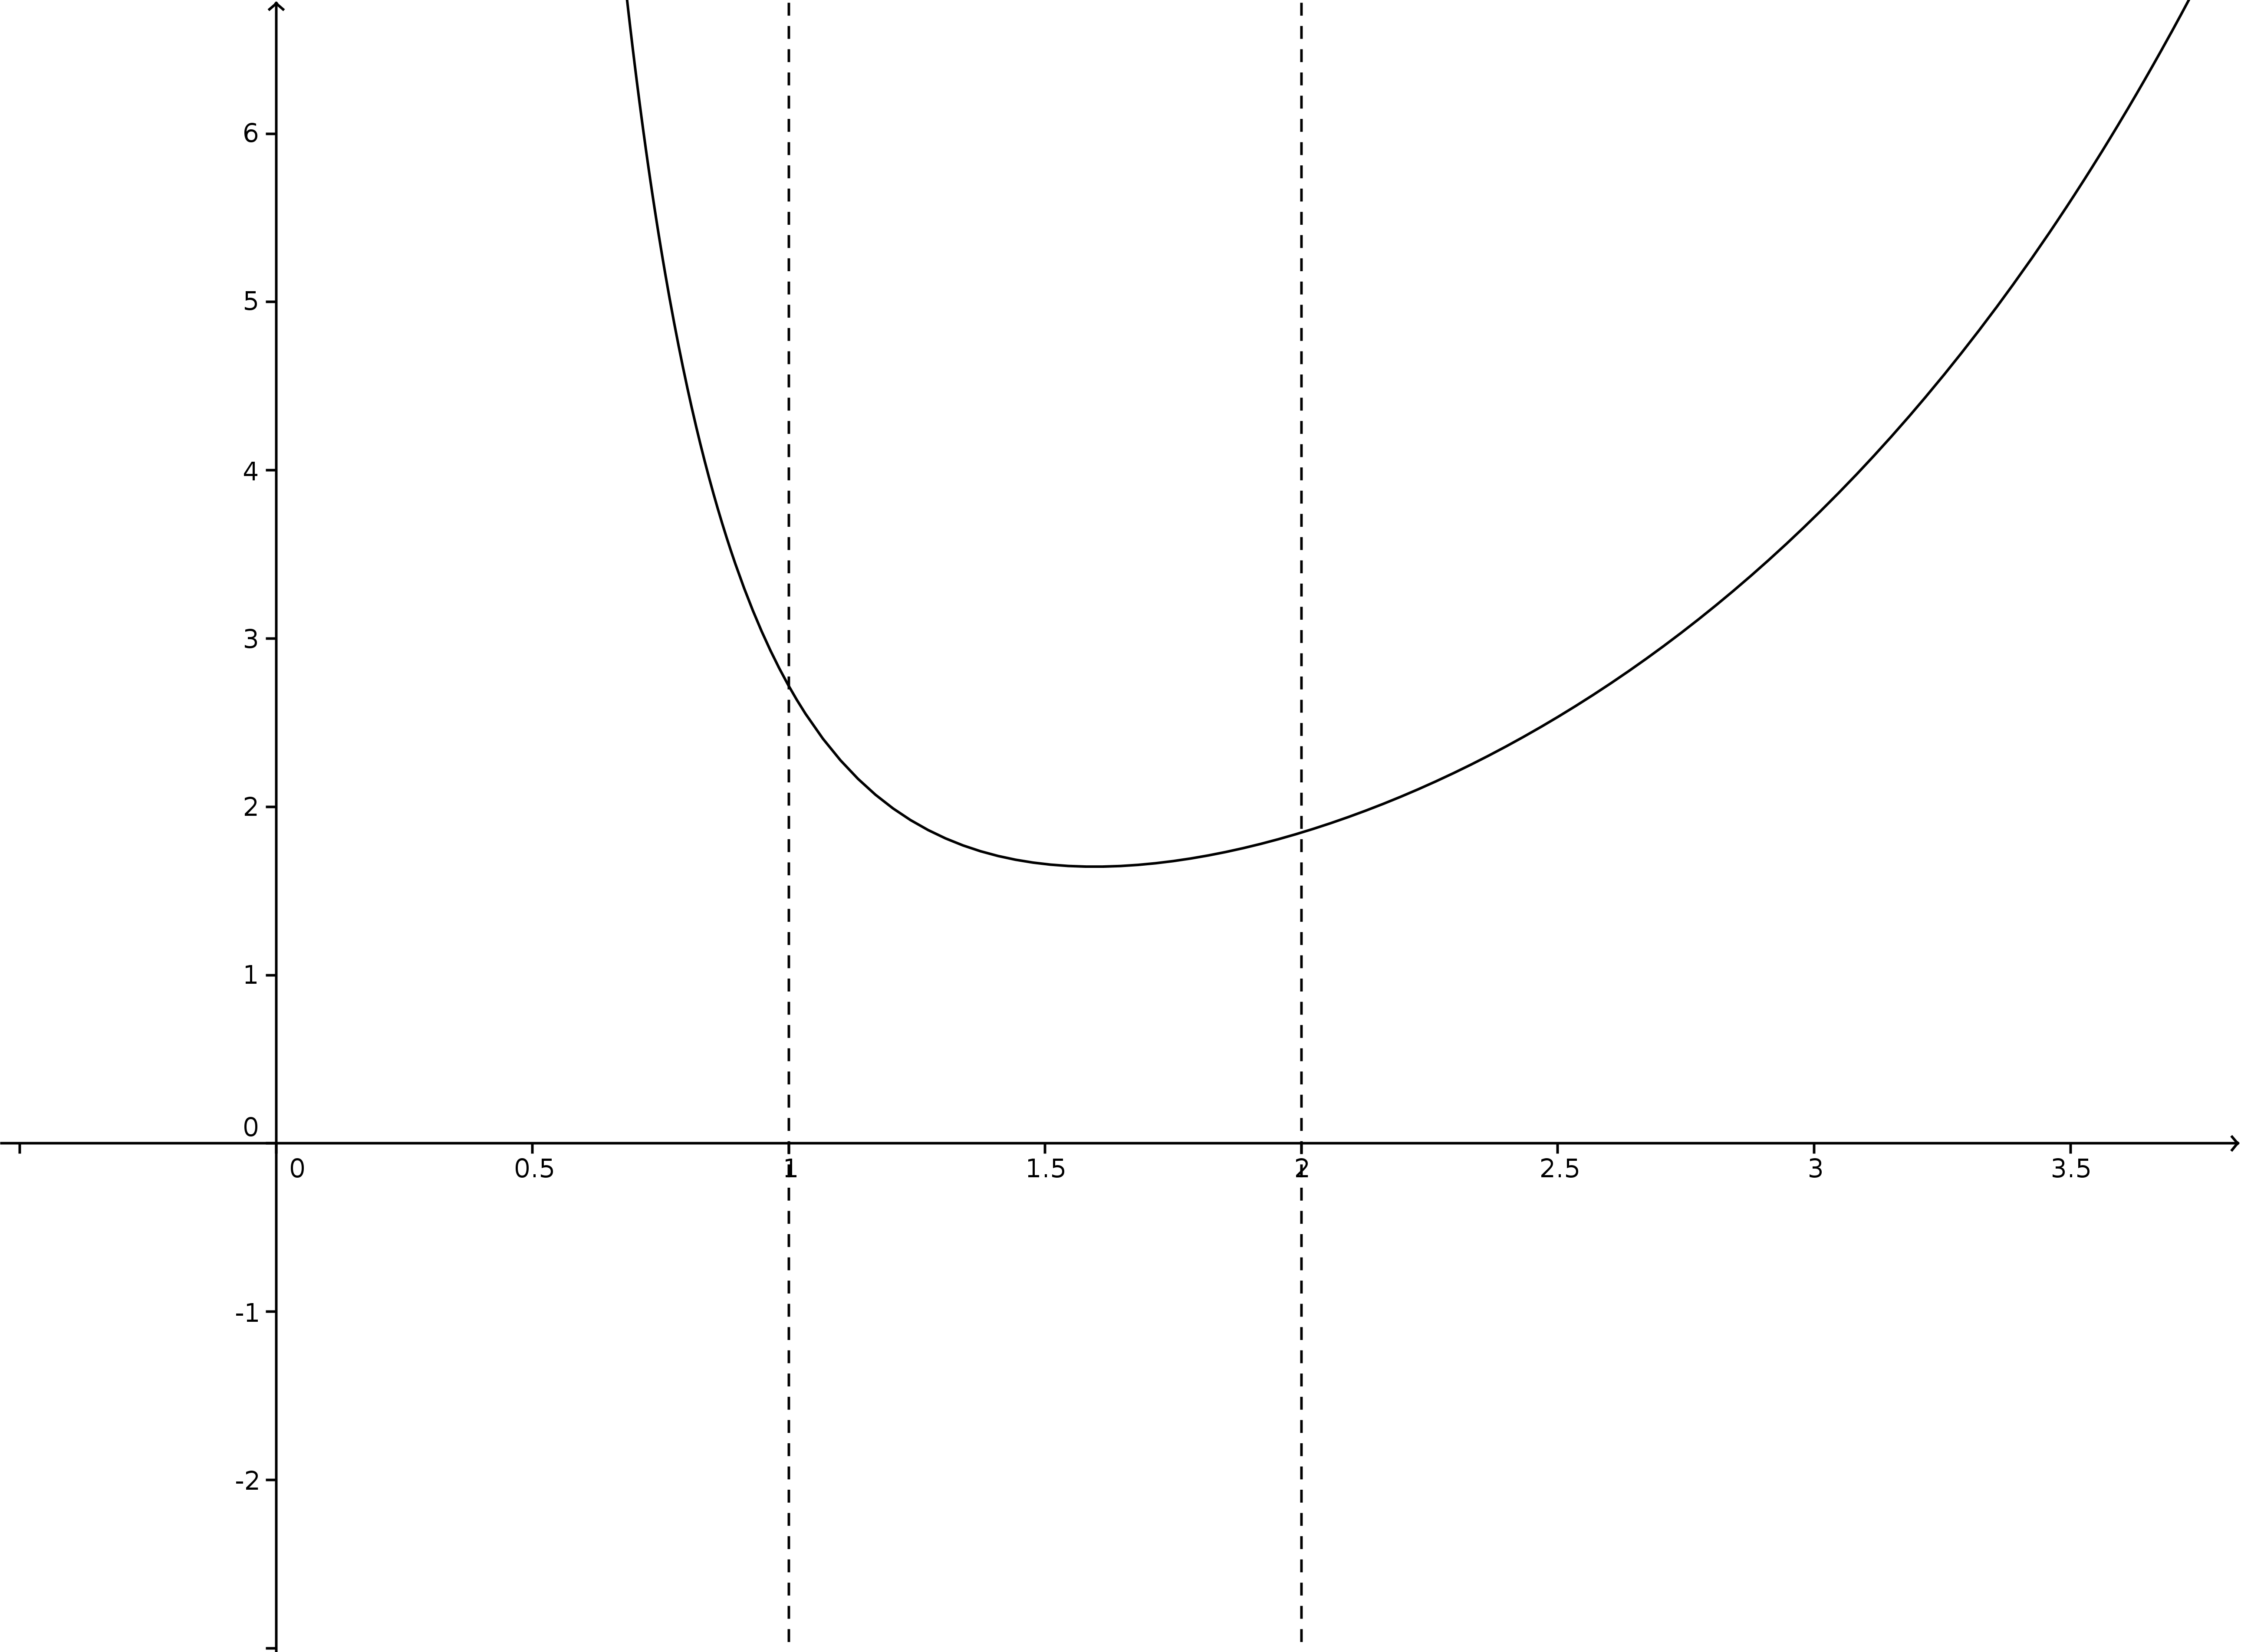
\includegraphics[scale=0.25]{ex08.png}
 			\caption{Gráfico de $f^{''}(x)$}
 		\end{figure}

		Através do gráfico vemos que o máximo ocorre em $x = 1$. Assim:

		\begin{align*}
		\begin{split}
		\max_{0 \leq t \leq 1} |f^{''}(t)| = |f^{''} (1)| &= 2.7182818\\
		\end{split}
		\end{align*}

		Portanto,

		\begin{align*}
		\begin{split}
		h^2  	&< \frac{0.05}{\frac{1}{12} \times 2.7182818 } \\
		h^2 	&< 0.22072766 \\
		h 		&< 0.46981662
		\end{split}
		\end{align*}

		Note que o espaçamento $h$ é dado por:

        \begin{align*}
		h = \frac{b - a}{N}
		\end{align*}

		onde $N + 1$ é a quantidade de pontos utilizados na aplicação da regra do Trapézio. Assim:

		\begin{align*}
		h = \frac{b - a}{N} < 0.46981662\implies N &> \frac{1}{0.46981662} \\
		N &> 2.12849  \\
		\end{align*}

		Logo devemos encontrar um valor $h$ tal que:

		\begin{align*}
		\frac{b - a}{h} = \frac{1}{h} = 3
		\end{align*}

		De fato,

		\begin{align*}
		\quad  h = 0.33333 < 0.46981
		\end{align*}

		Portanto um intervalo igualmente espaçado $h = 0.33333$ entre os pontos satisfaz o erro desejado num total de 4 pontos.

		\textbf{Cálculo da integral.}

		\hspace{2cm}

		\lstinputlisting[language=Python, caption= Cálculo em \textit{Python}, label=cod1]{algorithms/ex08-1.py}


		Executando o código acima obtemos $ 3.076079 $.


		\subsection{Exercício 9}

		Estamos interessados em obter um número mínimo de intervalos para o cálculo de

		\begin{align*}
			\int_{0}^{\frac{\pi}{2}} \euler^{-x}\cos(x)
		\end{align*}

		através da regra $ \frac{1}{3} $ de \textit{Simpson}, tal que o resultado obtido na integração tenha um erro menor que $10^{-5}$.

		Assim, devemos calcular o valor do espaçamento $h$ entre os pontos no cálculo, de forma a garantir o erro desejado.

		\begin{align*}
			\begin{split}
			| R(f) | \leq \frac{b - a}{180} \times h^4 \times \max_{a \leq t \leq b} |f^{iv}(t)| & < 10^{-5}\\ \implies \quad h^4  &< \frac{10^{-5}}{\frac{b - a}{180} \times \max_{a \leq t \leq b} |f^{iv}(t)|}
			\end{split}
		\end{align*}

		Onde $|f^{iv}(t)|$ é obtido fazendo:

		\begin{align*}
			\begin{split}
			f^{'} (x) &= -\euler^{-x}(\sin(x) + \cos(x)) \\
			f^{''} (x) &= 2\euler^{-x}\sin(x)\\
			f^{'''} (x) &= 2\euler^{-x}(\cos(x) - \sin(x))\\
			f^{iv} (x) &= -4\euler^{-x}\cos(x)\\
			\end{split}
		\end{align*}

		Através do gráfico vemos que o máximo de $|f^{iv}(x)|$ ocorre em $0$. Essa análise poderia ser feita observando que o produto $-4\euler^{-x}$ com $\cos(x)$ é mínimo quando $\euler^{-x}$ for mínimo, o que implica no maior valor absoluto possível de $f$ nesse intervalo ($\cos(x)$ é nulo em $\frac{\pi}{2}$).

 		\hspace{1cm}
		\begin{figure}[H]
			\centering
			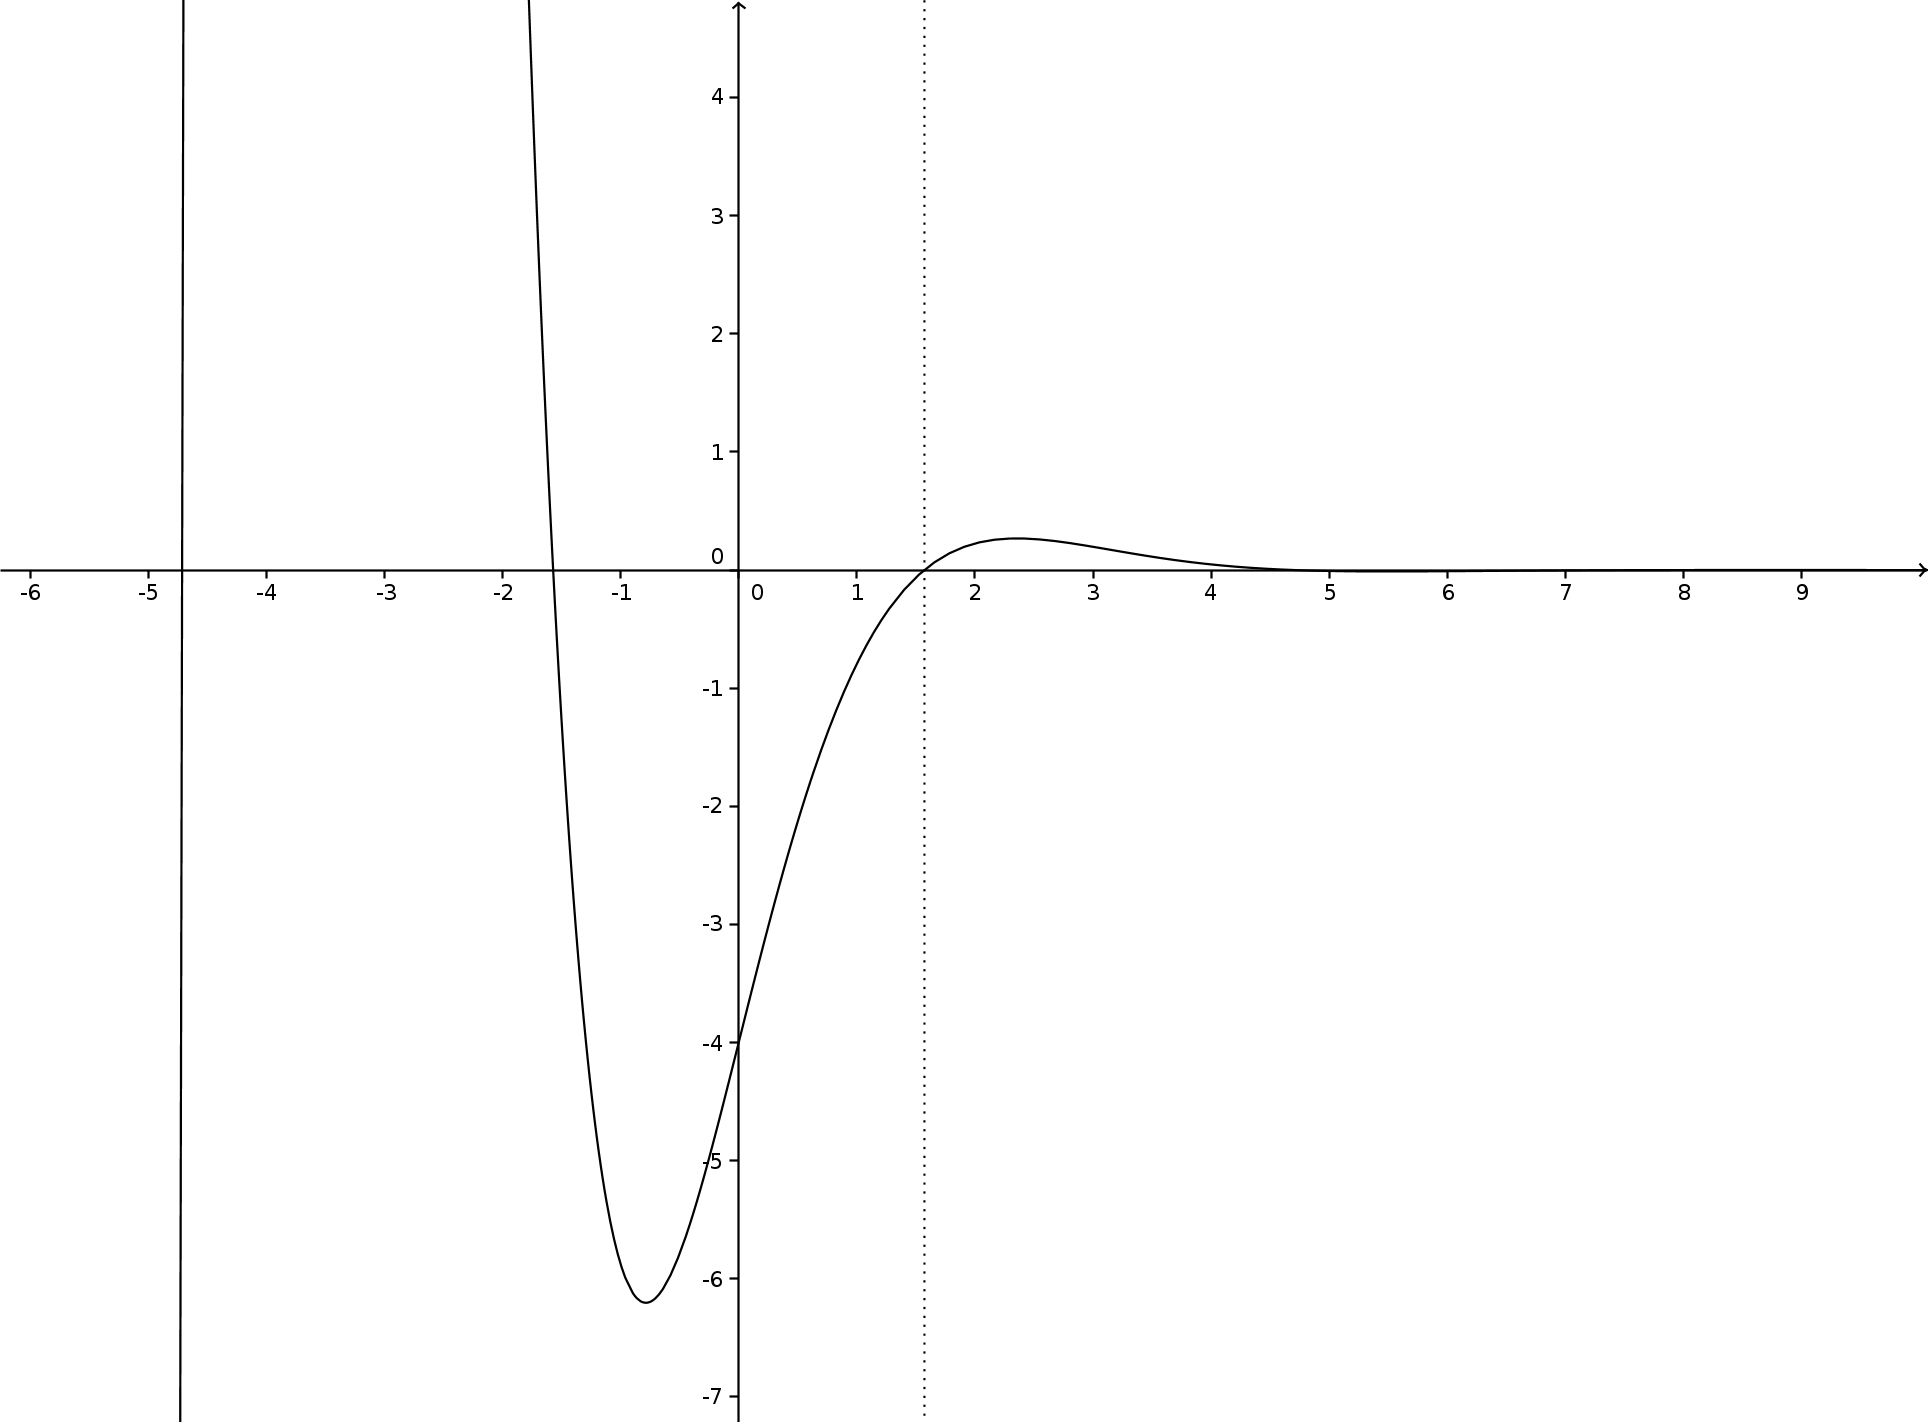
\includegraphics[scale=0.7]{e-xcos.png}
			\caption{Gráfico de $-4\euler^{-x}\cos(x)$}
		\end{figure}

		Continuando o cálculo de $h$ obtemos:

		\begin{align*}
			\begin{split}
			h^4  	&< \frac{10^{-5}}{\frac{b - a}{180} \times \max_{a \leq t \leq b} |f^{iv}(t)|} =  \frac{10^{-5}}{\frac{\frac{pi}{2} - 0}{180} \times |f^{iv}(0)|} = \frac{10^{-5}}{\frac{\pi}{90}} \\
			h^4		&<	0.00028647\\
			h			&< 0.13
			\end{split}
		\end{align*}

		Note que o espaçamento $h$ é dado por:

		\begin{align*}
			\begin{split}
				h = \frac{b - a}{2N}
			\end{split}
		\end{align*}

		e que o número de pontos necessários para aplicar a regra de $\frac{1}{3}$ de \textit{Simpson} é dado por $2N + 1$. Assim:

		\begin{align*}
		\begin{split}
		h = \frac{b - a}{2N} < 0.13 \implies 2N &>	\frac{\frac{\pi}{2}}{0.13}  \\														2N &> 12.0830486677
		\\														N	&>	6.04152433385					\\
		\end{split}
		\end{align*}

		Então um valor inteiro $  N = 7  $ satisfaz a condição, o que implica que devemos utilizar pelo menos $2N + 1 = 15$ pontos para garantir o erro desejado. Logo devemos utilizar um valor $h$ tal que:

		\begin{align*}
			h = \frac{\frac{\pi}{2}}{14} = 0.112199737629
		\end{align*}


		Portanto um intervalo igualmente espaçado $h = 0.112199737629$ entre os pontos satisfaz o erro desejado,em um total de $n = 15$ pontos.

		\textbf{Prova.} Calculando a integral analiticamente temos que:

		\begin{align*}
			\begin{split}
				\int \euler^{-x}cos(x)dx &= \euler^{-x}\sin(x) + \int \euler^{-x}\sin(x) dx \\ &= \euler^{-x}\sin(x) + \Big[ -\euler^{-x}\cos(x) - \int \euler^{-x}\cos(x) \Big] \\
				2\int \euler^{-x}cos(x)dx &= \euler^{-x}\sin(x) -\euler^{-x}\cos(x) \\
				\int \euler^{-x}cos(x)dx &= \frac{\euler^{-x}\sin(x) -\euler^{-x}\cos(x)}{2}
			\end{split}
		\end{align*}

		\begin{align*}
			\begin{split}
				\int_{0}^{\frac{\pi}{2}} \euler^{-x}cos(x)dx &=  \frac{\euler^{-x}\sin(x) -\euler^{-x}\cos(x)}{2} \Big|_{0}^{\frac{\pi}{2}} \\
				&= \frac{1}{2} \Big[ \euler{-\frac{\pi}{2}} -1 (-1) \Big] \\
				&= 0.60393978
			\end{split}
		\end{align*}

		E computacionalmente como segue:

		\hspace{2cm}

		\lstinputlisting[language=Python, caption= Cálculo em \textit{Python}]{algorithms/ex09-1.py}

		\hspace{2cm}

		\lstinputlisting[language=C, caption= Cálculo de integral pela regra 1/3 de \textit{Simpson} em \textit{C}]{algorithms/simpsonRule.c}


		Obtemos $ 0.603937665466 $ e $ 0.6039376655 $ respectivamente.

		\subsection{Exercício 10}

		Similar ao exercício anterior, queremos definir um intervalo $h$ de modo que a regra $\frac{3}{8}$ de \textit{Simpson} forneça um valor de $\int_{0.2}^{0.8}\sin(x)dx$ com um erro inferior a $0.5 \times 10^{-3}$.

		O valor de $h$ utilizando a regra $\frac{3}{8}$ de \textit{Simpson} é obtido fazendo:

		\begin{align*}
			\begin{split}
				| R(f) | \leq \frac{b - a}{80} \times h^4 \times \max_{a \leq t \leq b} |f^{iv}(t)| & < 0.5 \times 10^{-3}\\ \implies \quad h^4  &< \frac{0.5  \times 10^{-3}}{\frac{b - a}{80} \times \max_{a \leq t \leq b} |f^{iv}(t)|}
			\end{split}
		\end{align*}

		Assim,

	  \begin{align*}
		  \begin{split}
		  f^{'} (x) &= \cos(x)\\
		  f^{''} (x) &= -\sin(x)\\
		  f^{'''} (x) &= -\cos(x)\\
		  f^{iv} (x) &= \sin(x)\\
		  \end{split}
	  \end{align*}

		Onde $ \max_{0.2}^{0.8}|\sin(x)|$ ocorre em $0.8$. Logo:

		\begin{align*}
			\begin{split}
				h^4  	&< \frac{0.5  \times 10^{-3}}{\frac{b - a}{80} \times \max_{a \leq t \leq b} |f^{iv}(t)|} =  \frac{0.5  \times 10^{-3}}{\frac{0.8 - 0.2}{80} \times |f^{iv}(0.8)|} = \frac{0.5  \times 10^{-3}}{0.717356} \\
				h^4		&<	0.000697004\\
				h			&< 0.162483332738
			\end{split}
		\end{align*}

		Note que o espaçamento $h$ é dado por:

		\begin{align*}
			h = \frac{b-a}{3N}
		\end{align*}

		e que o número de pontos necessários para aplicar a regra de $\frac{3}{8}$ de \textit{Simpson} é dado por $3N + 1$. Portanto:

		\begin{align*}
		\begin{split}
			h = \frac{b - a}{3N} < 0.162483332738 \implies 3N &>	\frac{0.6}{0.162483332738}  \\														3N &> 3.692694
			\\														N	&>	1.260898					\\
		\end{split}
		\end{align*}

		Note que um valor inteiro $  N = 2  $ satisfaz a condição, então devemos utilizar pelo menos $3N + 1 = 7$ pontos para garantir o erro desejado. Logo devemos utilizar um valor $h$ tal que:

		\begin{align*}
			h = \frac{0.6}{6} = 0.1
		\end{align*}

		Portanto um intervalo igualmente espaçado $h = 0.1$ entre os pontos satisfaz o erro desejado, o que implica em uma quantidade de pontos $n = 7$ .

		\textbf{Prova.}
		Calculando analiticamente obtemos:

		\begin{align*}
			\begin{split}
				\int_{0.2}^{0.8}\sin(x) dx &= -\cos(x)\Big|_{0.2}^{0.8} \\
				&= -0.696706709347 - (-0.980066577841) \\ &= 0.283359868494
			\end{split}
		\end{align*}

		Calculando pela regra 3/8 de \textit{Simpson} temos que:
 		\begin{table}[H]
 			\def\arraystretch{1.5}
 			\begin{center}
 				\caption{Pontos $\sin(x)$}
 				\label{points_ex10}
 				\begin{tabularx}
 					{\textwidth}{|X|p{1.5cm}|p{1.5cm}|p{1.5cm}|p{1.5cm}|p{1.5cm}|p{1.5cm}|p{1.5cm}|}
 					\hline
 					{$x$} & 0.2 & 0.3 & 0.4 & 0.5 & 0.6 & 0.7 & 0.8 \\
 					\hline
 					{$f{(x)}$} & 0.198669 & 0.295520 & 0.389418 & 0.479425 & 0.564642 & 0.644217 & 0.71735\\
 					\hline
 				\end{tabularx}
 			\end{center}
 		\end{table}

		\begin{align*}
			\begin{split}
				\int_{0.2}^{0.8} \sin(x)  dx &= \frac{3h}{8}[ f(x_0) + 3[f(x_1) + f(x_2) + f(x_4) + f(x_5)] + 2f(x_3) + f(x_6)] \\
				&= \frac{0.3}{8}[0.198669 + 3(0.295520 + 0.389418 + 0.564642 + 0.644217) + 2(0.479425) \\ &+ 0.71735] \\
				&= \frac{0.3}{8}\left[0.916019 + 3(1.893797) + 0.95885\right]\\
				&= \frac{0.3}{8}\left[7.55626\right] \\
				&= 0.28335975\\
			\end{split}
		\end{align*}

		Observe que o erro obtido está em conformidade com o esperado.

		\subsection{Exercício 11}

		Estamos interessados em calcular $\Gamma(\alpha) = \int_{0}^{\infty} \euler^{-x}x^{\alpha-1} dx$ com $\alpha = 5$, através da Quadratura de Gauss.

		Note que o intervalo de integração e a função peso coincidem com o polinômio ortogonal de \textit{Laguerre}. Os polinômios ortogonais de  \textit{Laguerre} são obtidos através do produto escalar:

		\begin{align*}
		\begin{split}
			(f, g) = \int_{0}^{+\infty} \euler^{-x} f(x)g(x) dx
		\end{split}
		\end{align*}

		Iremos calcular a integral $ \int_{0}^{\infty} \euler^{-x}x^{4} dx $ utilizando um polinômio de grau três, onde os valores de $x_i$ e $A_i$ são dados por:

		\begin{align*}
		\begin{split}
			x_0 = 0.4157745567 	&\quad\quad A_0 = 0.7110930099 	\\
			x_1 = 2.294280360		&\quad\quad A_1 = 0.2785177335	\\
			x_2	=	6.289945082		&\quad\quad	A_2	=	0.01038925650
		\end{split}
		\end{align*}

		Logo,

		\begin{align*}
		\begin{split}
			\int_{0}^{\infty} \euler^{-x}x^{4} dx &= A_0f(x_0) + A_1f(x_1) + A_2f(x_2) \\&=  0.7110930099 \times (0.4157745567)^4 + 0.2785177335 \times (2.294280360)^4 \\&+ 0.01038925650	 \times (6.289945082)^4 \\
			&= 0.0212499565433 + 6.8806059301 + 16.2619223537 \\
			&= 23.1637782403
		\end{split}
		\end{align*}

		\section*{Lista de Exercícios 6}

		\subsection{Exercício 1}

		\textbf{a)} Dado o problema de valor inicial abaixo, queremos encontrar uma aproximação para $y(5)$ usando o método de Euler melhorado.

		\[
		\begin{cases}
		\ y^{'} &= \quad 4 - 2x\\

		\ y(0) &= \quad 2\\
		\end{cases}
		\]

		Dado o método de Euler melhorado:

		\begin{align*}
				y_{n + 1} = y_n + \frac{h}{2}(k_1 + k_2)
		\end{align*}

		onde,

		\begin{align*}
			\begin{split}
				k_1 &= f(x_n, y_n) \\
				k_2 &= f(x_n + h, k_1\times h + y_n))
			\end{split}
		\end{align*}

		Através do seguinte algoritmo em \textit{Python}:

		\hspace{2cm}

		\lstinputlisting[language=Python, caption= {Cálculo do P.V.I em \textit{Python} com h = 0.5}]{algorithms/ex01-2_h05.py}

		\hspace{2cm}

		\lstinputlisting[language=Python, caption= {Cálculo do P.V.I em \textit{Python} com h = 0.25}]{algorithms/ex01-2_h025.py}

		\hspace{2cm}

		\lstinputlisting[language=Python, caption= {Cálculo do P.V.I em \textit{Python} com h = 0.125}]{algorithms/ex01-2_h0125.py}

		Obtemos os resultados para h = 0.5, h = 0.25 e h = 0.125 respectivamente, como segue:
		\hspace{2cm}

		\VerbatimInput{algorithms/output/ex01-2_h05.txt}

		\hspace{2cm}

		\VerbatimInput{algorithms/output/ex01-2_h025.txt}

		\hspace{2cm}

		\VerbatimInput{algorithms/output/ex01-2_h0125.txt}

		Logo a resolução para o P.V.I em $ y(5) $ é igual a $-3$.

		\textbf{b)} A equação diferencial é do tipo separável, portanto podemos obter a solução geral como se segue:

		\begin{align*}
		\begin{split}
			\frac{dy}{dx} &= 4 - 2x\\
			\int dy &= \int 4 - 2x dx \\
			y &= 4x - x^2 + C
		\end{split}
		\end{align*}

		\begin{align*}
			C = x^2 - 4x + y \implies C = (0)^2 - 4(0) + 2 = 2
		\end{align*}

		Portanto a solução exata para o P.V.I. pode ser obtida:

		\begin{align*}
			y(5) = 4(5) - (5)^2 + 2 = -3
		\end{align*}

		Exatamente o mesmo valor obtido nos algoritmos com os espaçamentos 0.5, 0.25 e 0.125 .

		\subsection{Exercício 2}

		Dado o P.V.I. abaixo, estamos interessados em calcular uma aproximação para y(16), por Runge-Kutta de segunda ordem e Runge-Kutta de quarta ordem.

		\[
		\begin{cases}
		\ y' &= \quad \frac{-x}{y}\\

		\ y(0) &= \quad 20\\
		\end{cases}
		\]

		\textbf{a)} Por Runge-Kutta de segunda ordem, aplicamos:

		\hspace{2cm}

		\lstinputlisting[language=Python, caption= {Cálculo do P.V.I em \textit{Python} com h = 2}]{algorithms/ex02a-2_h2.py}

		\hspace{2cm}

		\VerbatimInput{algorithms/output/ex02a-2_h2.txt}

		\lstinputlisting[language=Python, caption= {Cálculo do P.V.I em \textit{Python} com h = 1}]{algorithms/ex02a-2_h1.py}

		\hspace{2cm}

		\VerbatimInput{algorithms/output/ex02a-2_h1.txt}

		\textbf{b)} O método de Runge Kutta de quarta ordem é dado por:

		\begin{align*}
			y_{n + 1} = y_n + \frac{h}{6}(k_1 + 2(k_2 + k_3) + k_4)
		\end{align*}

		onde,

		\begin{align*}
			\begin{split}
				k_1 &= f(x_n, y_n) \\
				k_2 &= f(x_n + \frac{1}{2}h,\ \frac{1}{2}hk_1 + y_n))\\
				k_3 &= f(x_n + \frac{1}{2}h,\ \frac{1}{2}hk_2 + y_n))\\
				k_4 &= f(x_n + h,\ y_n + hk_3) \\
			\end{split}
		\end{align*}


		Por Runge-Kutta de quarta ordem, aplicamos os seguintes algoritmos em \textit{Python}:

		\hspace{2cm}

		\lstinputlisting[language=Python, caption= {Cálculo do P.V.I. com h = 4}]{algorithms/ex02b-2_h4.py}

		\lstinputlisting[language=Python, caption = {Cálculo do P.V.I. com h = 2}]{algorithms/ex02b-2_h2.py}

		Onde obtemos:

		\VerbatimInput{algorithms/output/ex02b-2_h4.txt}

		\VerbatimInput{algorithms/output/ex02b-2_h2.txt}


		\subsection{Exercício 3}

		Dado o P.V.I:

		\[
		\begin{cases}
		\ y^{'} &= \quad yx^2 - y\\

		\ y(0) &= \quad 1\\
		\end{cases}
		\]

		Cuja solução analítica é:

		\begin{align*}
			\begin{split}
				\frac{dy}{dx} &= yx^2 - y \\
				\frac{dy}{dx} &= y(x^2 - 1) \\
				\frac{dy}{y} &= (x^2 - 1)dx \\
				\int \frac{dy}{y} &= \int (x^2 - 1)dx \\
				\ln(y) &= \frac{1}{3}x^3 - x + C \\
				\euler^{\ln(y)} &= \euler^{\frac{1}{3}x^3 - x }+ C \\
				y &= \euler^{\frac{1}{3}x^3 - x } + C
			\end{split}
		\end{align*}

		\begin{align*}
			C = y - \euler^{\frac{1}{3}x^3 - x }+ C  \implies C = 1 - \euler^{0} = 0
		\end{align*}

		\textbf{a)} Podemos calcular a solução aproximada pelo método de Euler, ou seja, pelo método de Taylor de ordem 1, onde:

		\begin{align*}
			y_{n + 1} = y_n + h \times f_n \\
		\end{align*}

		\begin{align*}
			%f_n = y'x^2 + 2xy - y' \quad y' = yx^2 -y\\
			f_n = yx^2 - y
		\end{align*}

%		\begin{align*}
%			\begin{split}
%			  f_n &= (yx^2 -y)x^2 + 2xy - (yx^2 -y) \\
%			\end{split}
%		\end{align*}

		\hspace{1.5cm}
		Assim, ao passo de h = 0.25 em [0, 2] temos:
		\hspace{1.5cm}

		$	n = 0	$

		\begin{align*}
			\begin{split}
				y_1 &= 	y_0 + 0.25(f_0) \\
						&=	1	+ 0.25[(1)(0) + 2(1)(0) - (1)] \\
						&=	0.75
			\end{split}
		\end{align*}

		$	n = 1	$

		\begin{align*}
		\begin{split}
		y_2 	&= 	y_1 + 0.25(f_1) \\
					&= 	0.75 + 0.25((0.75)(0.0625) - (0.75) \\
					&=	0.57421875
		\end{split}
		\end{align*}

		$\ldots$

		Calculemos todas as iterações através do seguinte algoritmo:

		\hspace{2cm}

		\lstinputlisting[language=Python, caption= {Cálculo do P.V.I. com h = 0.25}]{algorithms/ex03a-2_h025.py}

		Onde obtemos:

		\VerbatimInput{algorithms/output/ex03a-2_h025.txt}

		\textbf{b)} A solução aproximada pelo método de Euler melhorado, com h = 0.25 em [0, 2] é obtida executando:

		\hspace{2cm}

		\lstinputlisting[language=Python, caption= {Cálculo do P.V.I. com h = 0.25}]{algorithms/ex03b-2_h025.py}

		Onde obtemos:

		\VerbatimInput{algorithms/output/ex03b-2_h025.txt}

		\textbf{c)} Pelo método de Runge Kutta de quarta ordem, temos:

		\hspace{2cm}

		\lstinputlisting[language=Python, caption= {Cálculo do P.V.I. com h = 0.25}]{algorithms/ex03c-2_h025.py}

		Onde obtemos:

		\VerbatimInput{algorithms/output/ex03c-2_h025.txt}

		\textbf{d)}

 		\begin{figure}[H]
 			\centering
 			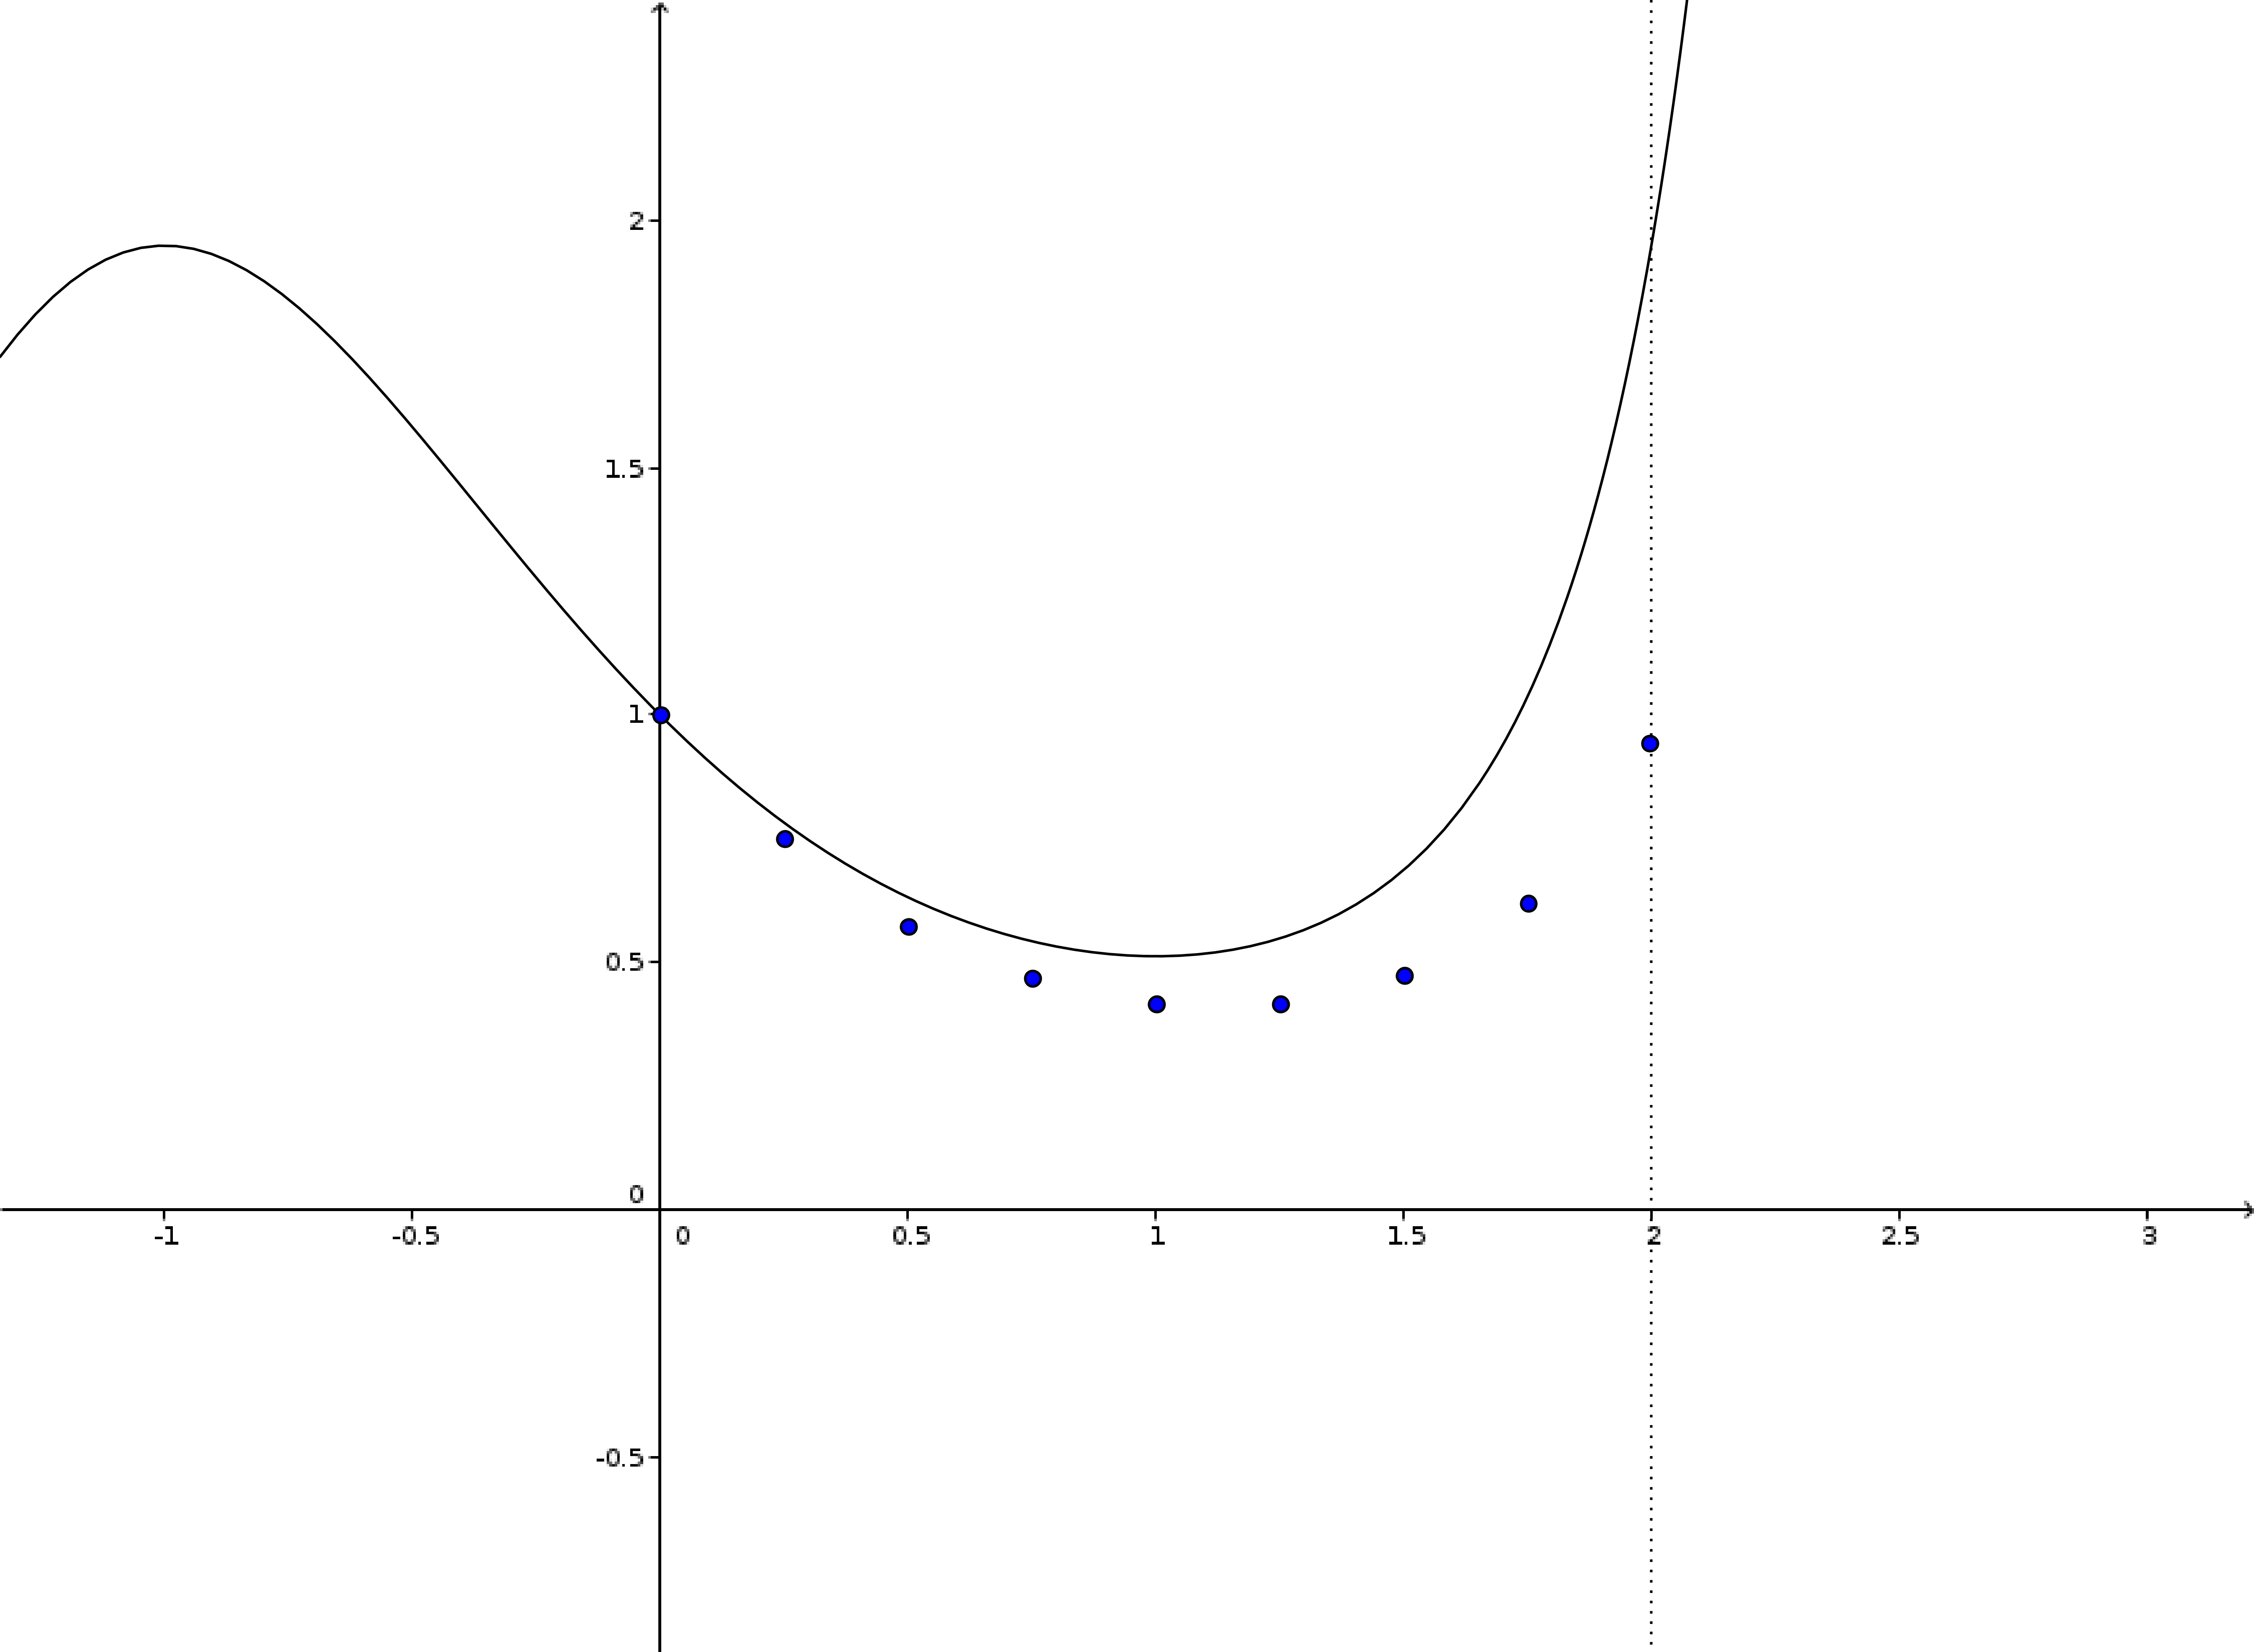
\includegraphics[scale=0.25]{grafedo1.png}
 			\caption{Pontos obtidos no método de Taylor de grau 1 e solução exata}
 		\end{figure}

 		\begin{figure}[H]
 			\centering
 			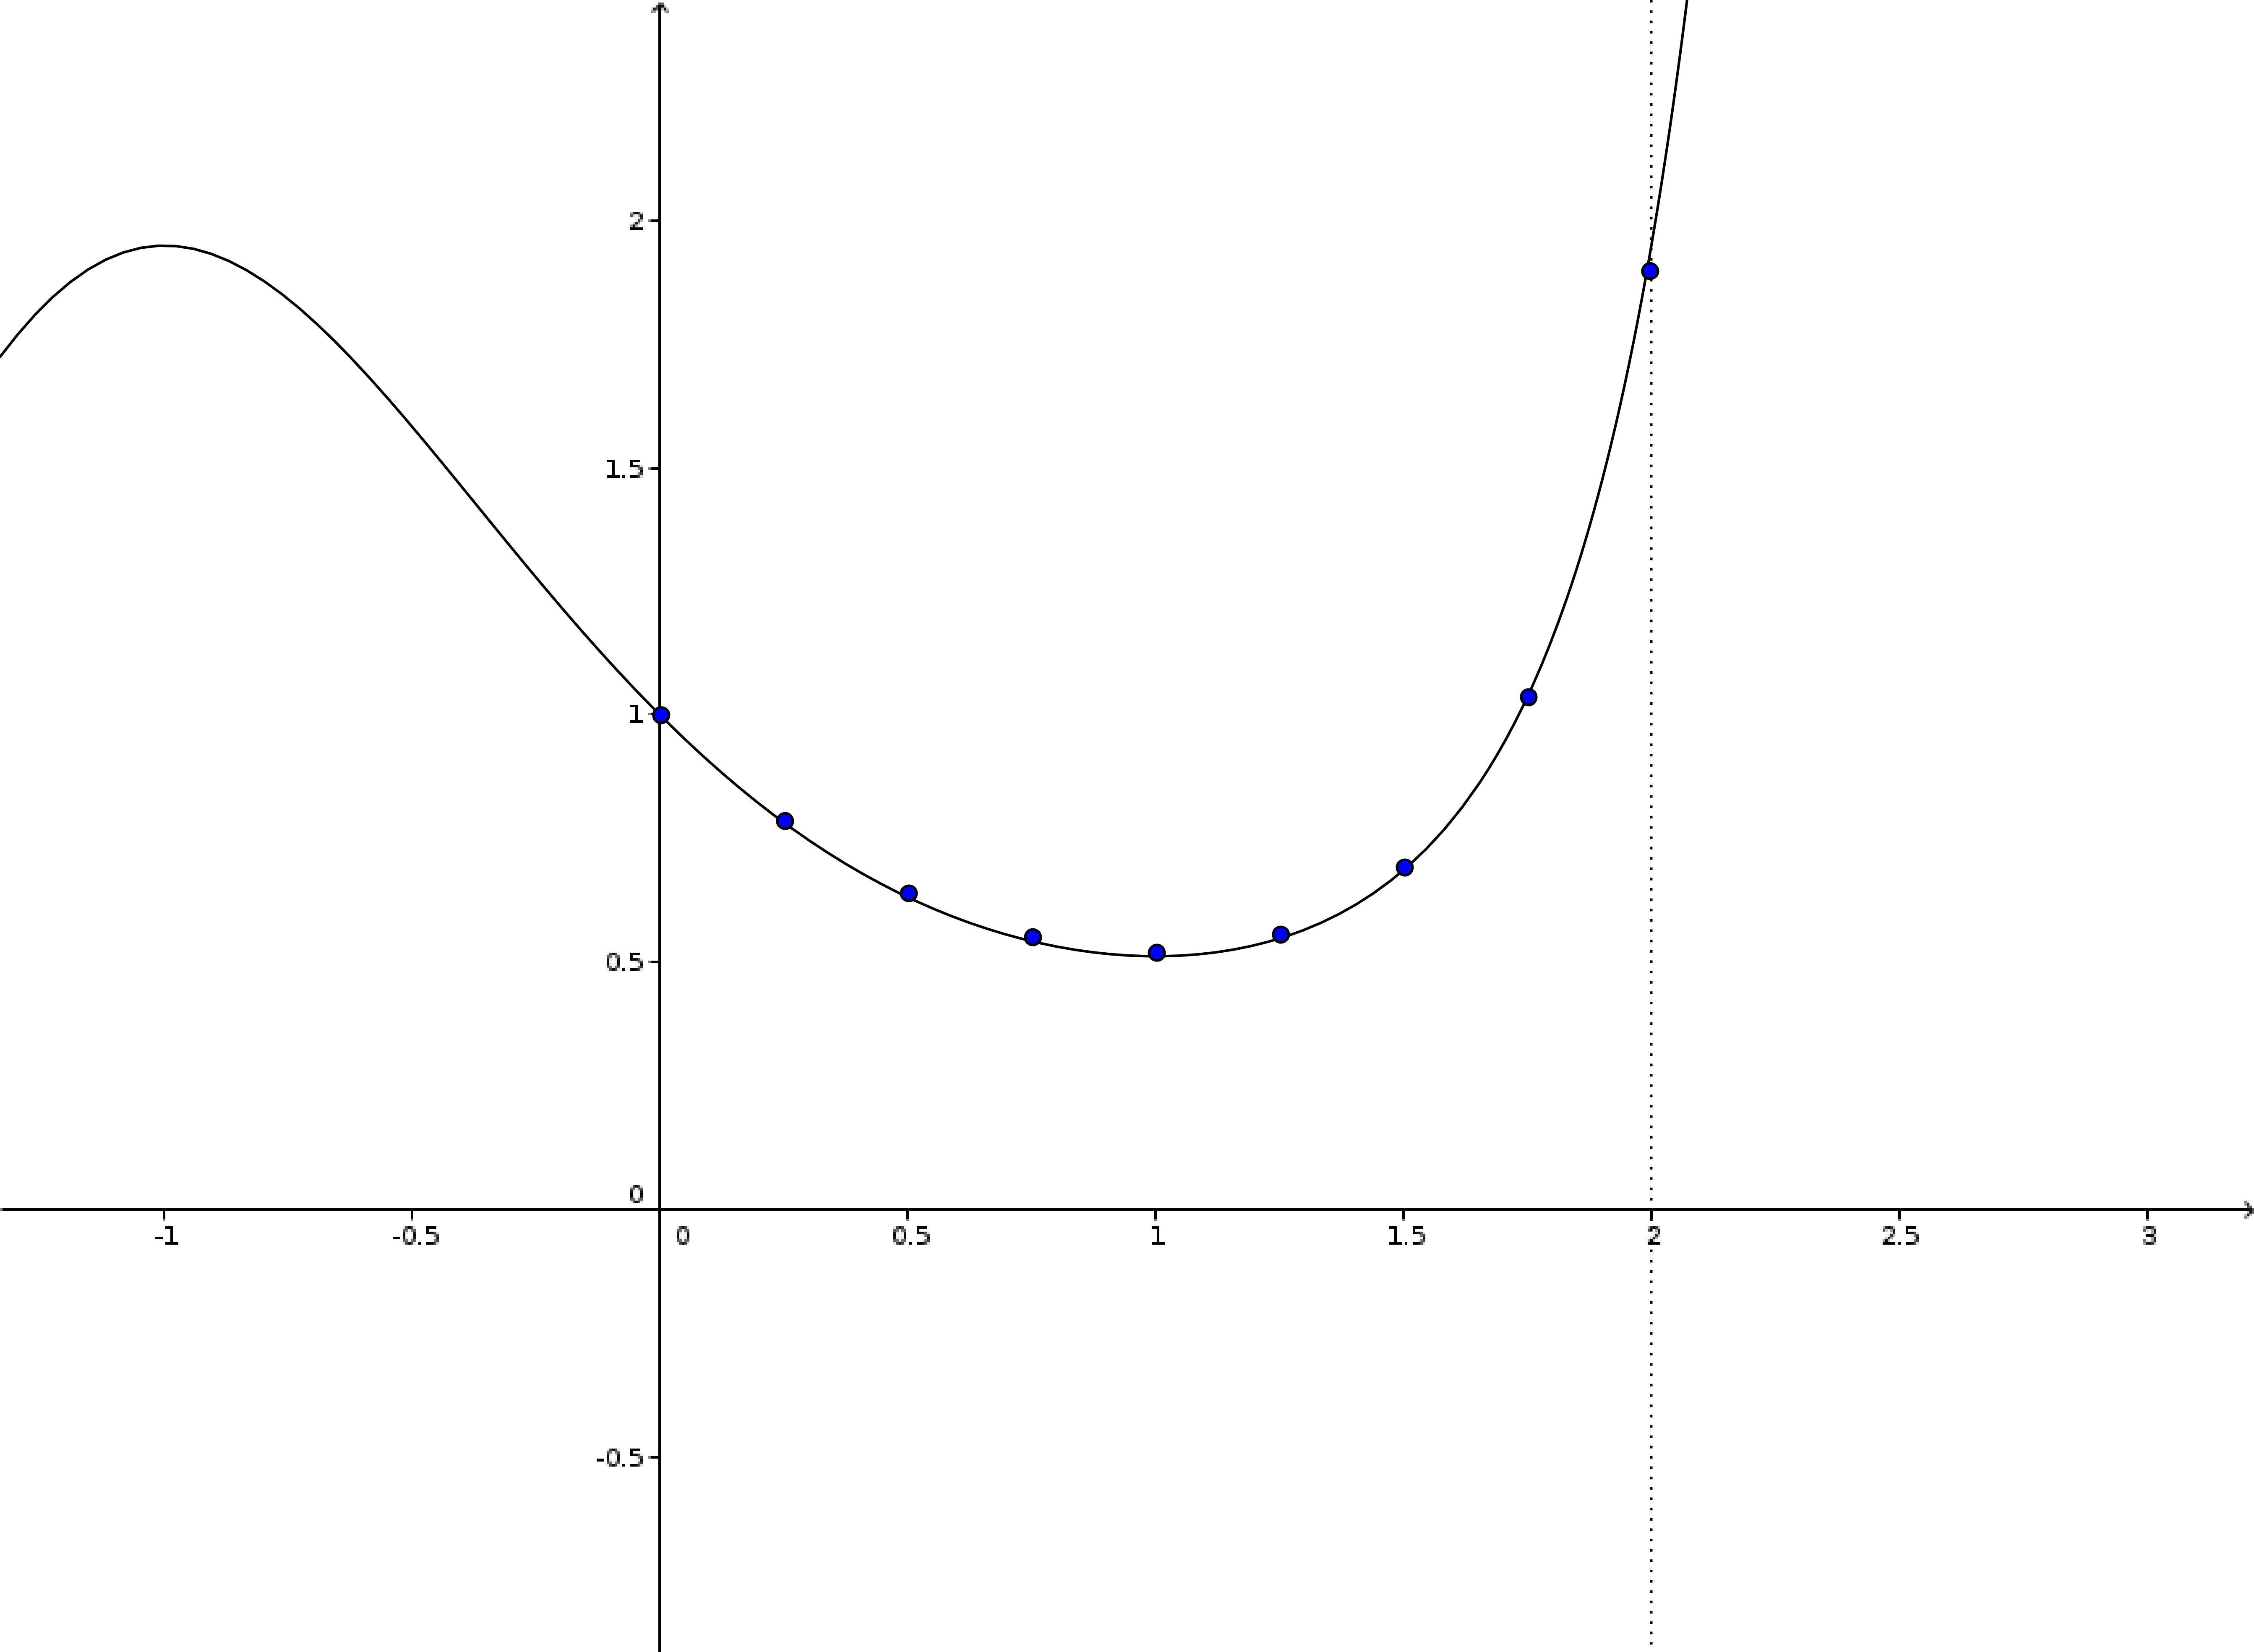
\includegraphics[scale=0.25]{grafedo2.png}
 			\caption{Pontos obtidos no método de Euler melhorado e solução exata}
 		\end{figure}

 		\begin{figure}[H]
 			\centering
 			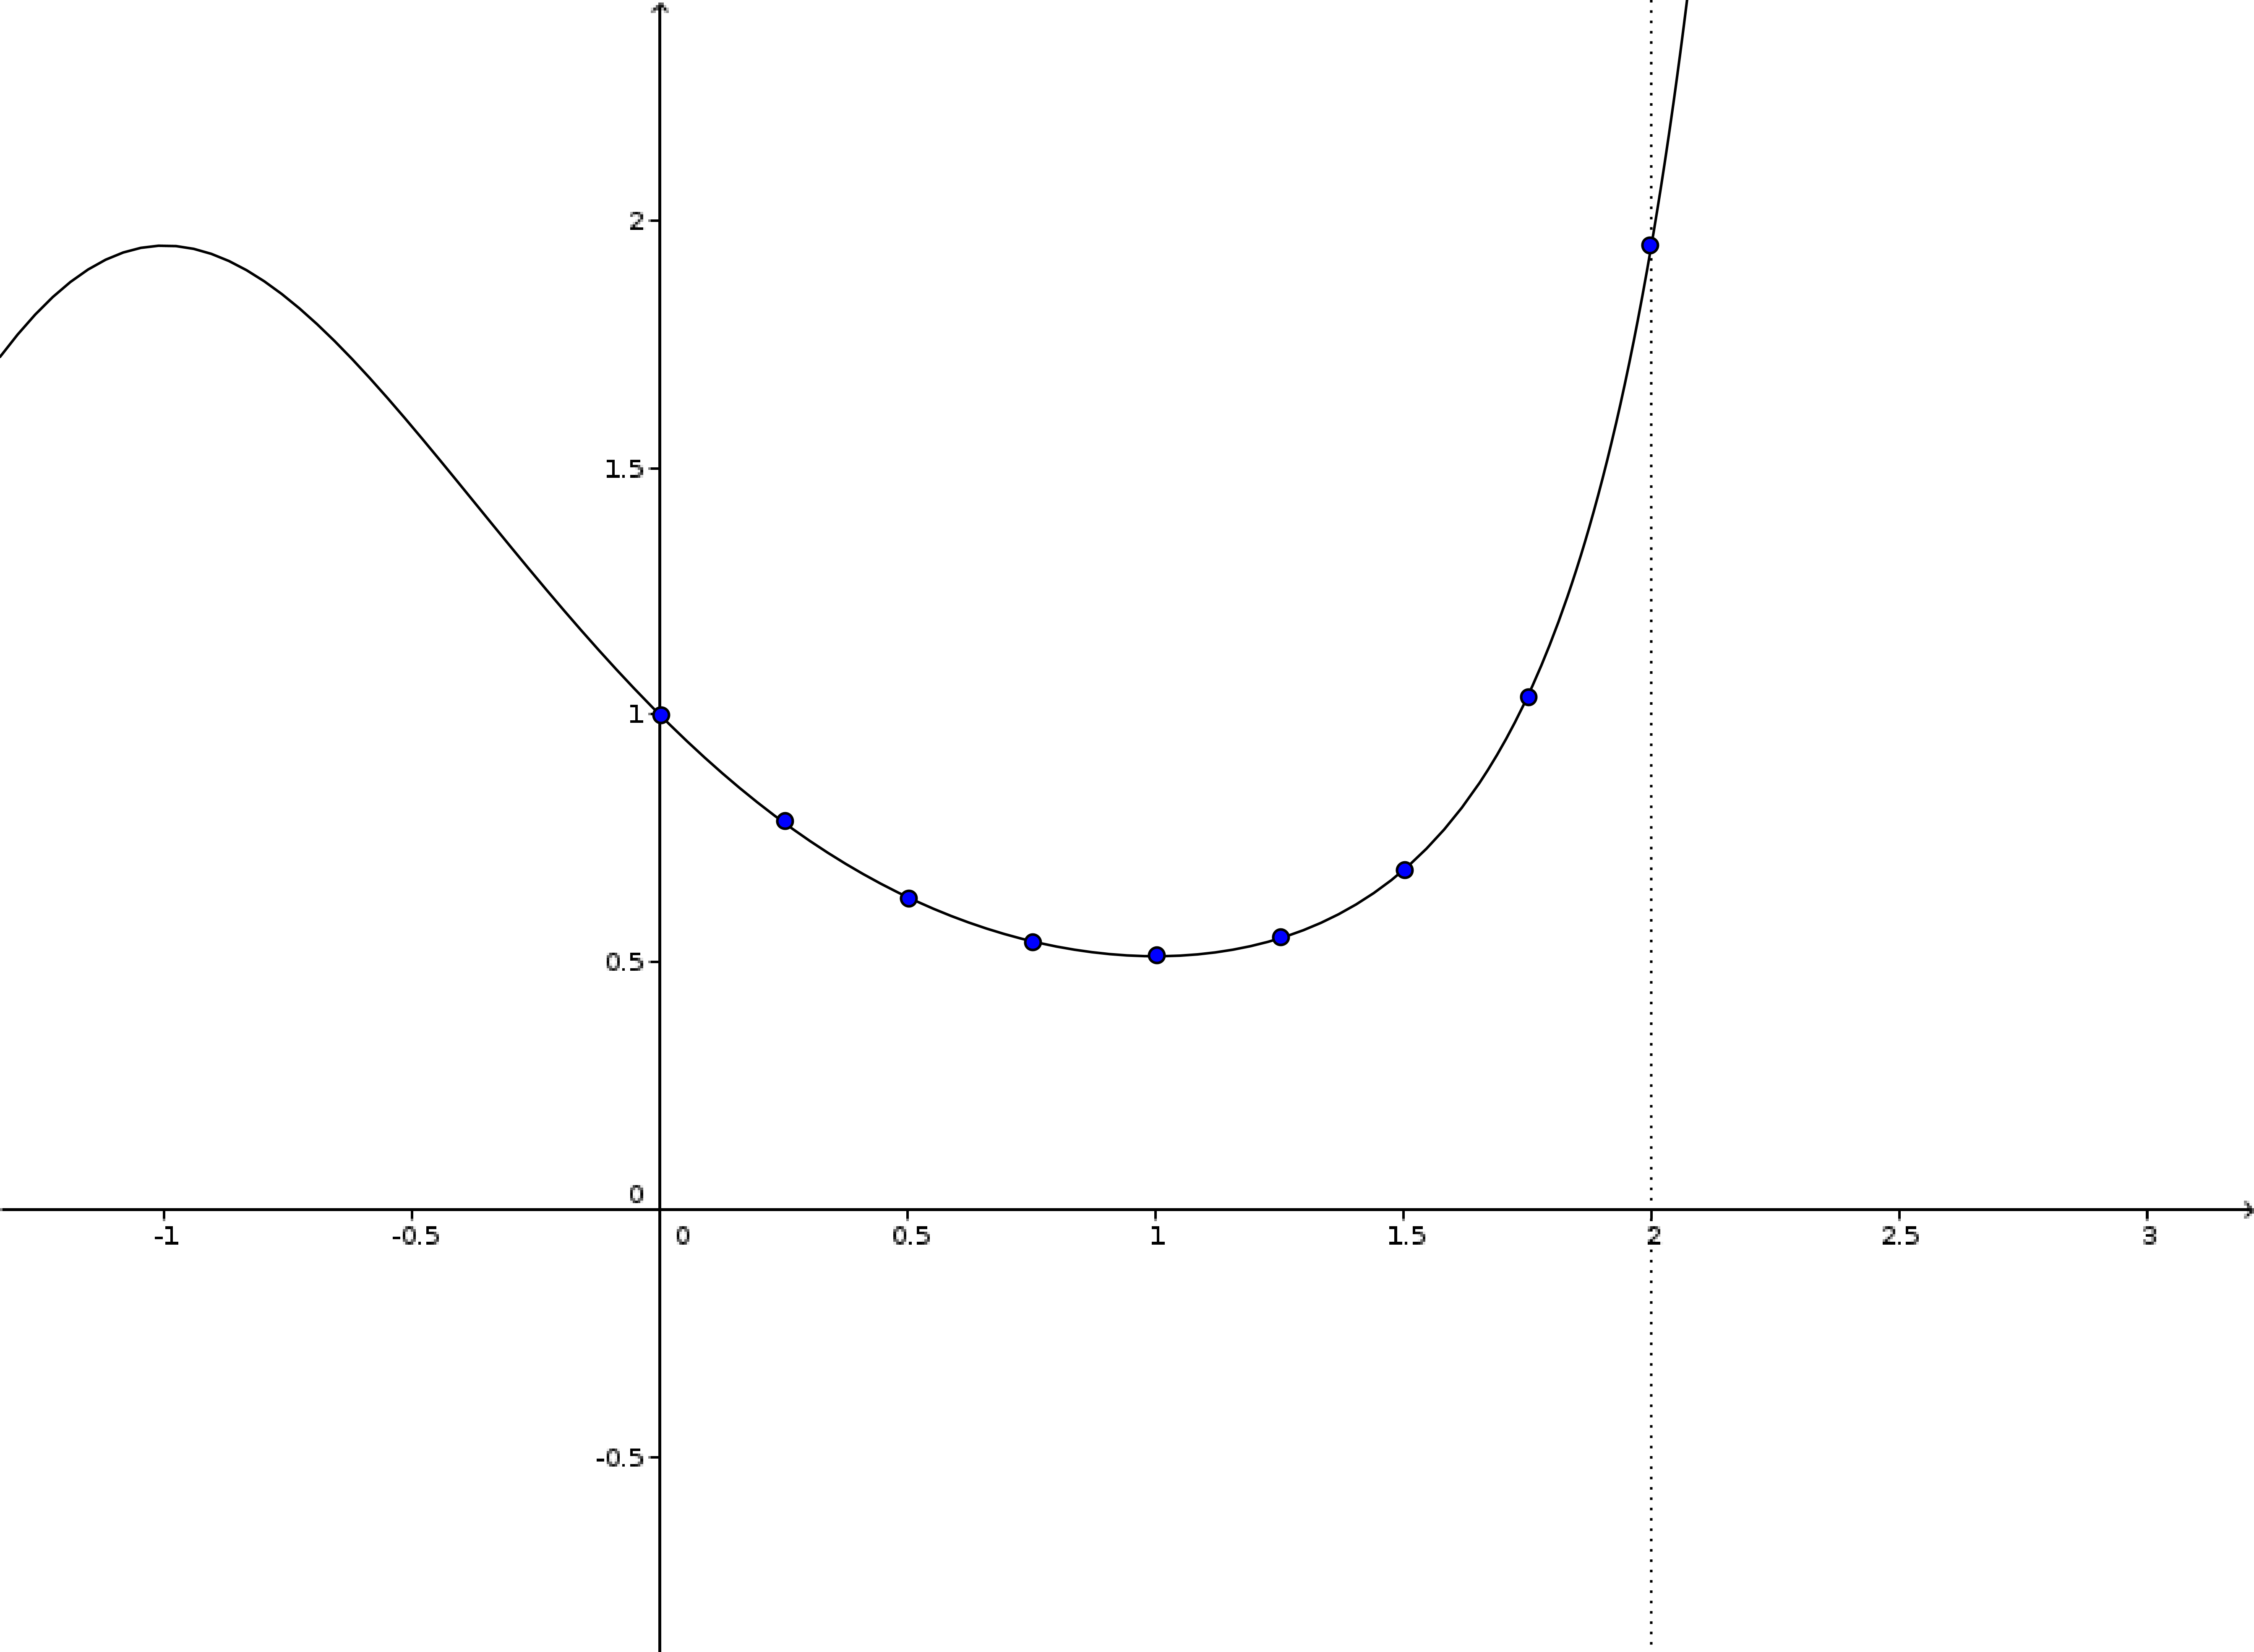
\includegraphics[scale=0.25]{grafedo3.png}
 			\caption{Pontos obtidos no método de Runge Kutta de quarta ordem e solução exata}
 		\end{figure}

		\subsection{Exercício 4}

		Queremos encontrar a fórmula de Taylor de ordem 2 para o P.V.I.

		\[
		\begin{cases}
		\ y' + y &= \quad x \\
		\ y(0) &= \quad 0\\
		\end{cases}
		\]

		com h = 0.1

		A fórmula de Taylor de segunda ordem é da forma:

		\begin{align*}
			\begin{split}
				y_{n + 1} = y_n + (h\times f_n) + (\frac{h^2}{2} \times f_n')
			\end{split}
		\end{align*}

		onde,

		\begin{align*}
			\begin{split}
				f_n &= x - y \\
				f_n' &= 1 - y' \\
						&= 1 - x + y \\
			\end{split}
		\end{align*}

		Portanto,

		\begin{align*}
			\begin{split}
				y_{n + 1} = y_n + (0.1\times (x_n - y_n)) + (0.05 \times (1 - x_n + y_n)) \\
			\end{split}
		\end{align*}

		\textbf{b)} De fato $y(x) = \euler^{-x} +x - 1$ é solução do P.V.I. pois:

		\begin{align*}
			y(0) = \euler^0 + 0 - 1 = 0 \\
		\end{align*}

		e,

		\begin{align*}
			\begin{split}
				y' = -\euler^{-x} + 1 \implies (-\euler^{-x} + 1) + \euler^{-x} +x - 1 &= x \\
			\end{split}
		\end{align*}

		\subsection{Exercício 5}

		Estamos interessados em resolver o P.V.I.

		\[
		\begin{cases}
		\ xy' - x^2y - 2&= \quad 0 \\
		\ y(1) &= \quad 3 \\
		\end{cases}
		\]

		$\forall x \in [1, 2]$

		E encontrar uma solução aproximada em $x = 1.5$, através do método de Euler melhorado e o Runge Kutta de quarta ordem.

		Assim, definimos um intervalo h para que a solução em 1.5 seja definida, e isolamos a função para utilizar os métodos como segue:

		\begin{align*}
			y' = \frac{2 + x^2y}{x}
		\end{align*}

		Executando os códigos abaixo:

		\hspace{2cm}

		\lstinputlisting[language=Python, caption= {Cálculo do P.V.I. com h = 0.25}]{algorithms/ex05-2-euler.py}

		\lstinputlisting[language=Python, caption= {Cálculo do P.V.I. com h = 0.25}]{algorithms/ex05-2-rt.py}

		Obtemos como soluções:

		\VerbatimInput{algorithms/output/ex05-2-euler.txt}

		\VerbatimInput{algorithms/output/ex05-2-rt.txt}

\end{document}
